This chapter explores the concept of Retroactive Call Subsumption (RCS). RCS
enables full sharing of answers among subgoal calls, independent of the order they are called,
using the relation of subsumption.

We start by introducing the motivations behind RCS by illustrating the shortcomings of traditional call
subsumption mechanisms. Next, we present the concepts introduced by RCS and how execution
rules are extended to support retroactive-based tabling. Other extensions are then discussed, namely:
the new table space organization based around the ideas of the \textit{common global trie} proposal
\cite{CostaJ-08} and the algorithm to traverse the subgoal trie to search for subsumed subgoals. Finally, we
give some details about the implementation of this new extension in the YapTab system.

\section{Motivation}

In traditional call subsumption, a new call to the subgoal $G$ is considered a generator subgoal
when a more general subgoal $G'$ is not found on the subgoal trie and it is the first time $G$ is called.
When $G'$ exists, $G$ is considered a consumer subgoal and a new consumer node is allocated to consume
answers from the subsuming subgoal $G'$.

Consider that the subgoal \texttt{p(X,1,2)} is called first, followed by \texttt{p(X,1,Z)}.
Notice that when \texttt{p(X,1,2)} is called, it is considered a generator subgoal as no subsuming subgoals
are found on the subgoal trie. The subgoal \texttt{p(X,1,Z)} is also considered a generator, because
\texttt{p(X,1,2)} does not subsume \texttt{p(X,1,Z)}. If the call order is swapped, \texttt{p(X,1,Z)} continues
to be considered a generator subgoal, but now \texttt{p(X,1,2)} finds \texttt{p(X,1,Z)} as a subsuming subgoal
on the subgoal trie, and thus is considered a consumer subgoal.

While call subsumption provides good results in terms of memory utilization and time it suffers from a
major problem: the order in which the the subgoals are called can greatly affect the performance
and applicability of the technique. Therefore, we introduce a new mechanism called \textit{Retroactive Call
Subsumption} (RCS) that solves the problem by retroactively modifying active tabled nodes to enable full sharing
of answers between subsuming and subsumed subgoals, independently of the order they are called.
Please notice that retroactive-based tabling is to be used with batched scheduling only.

\section{General Idea}

Retroactive Call Subsumption is based around the idea of stopping the computation of subsumed subgoals
that are currently running by transforming those generator subgoals into consumer subgoals, thus instead
of generating their own answers by means of code execution, they will consume answers from the more general
subgoal that has been called.

When the generator subgoal $G$ executes, an arbitrary number of choice points are created that are directly related
to $G$, that is, they are used to compute $G$'s answers. Therefore, when $G$
must be transformed into a consumer subgoal we must \textit{selectively prune} the parts of the computation
that are related to $G$ and transform $G$'s generator choice point in such a way that the choice point
will consume answers from its generator subgoal, instead of generating its own answers.
Pruning the computation of $G$ can thus potentially save execution time as $G$ no longer properly executes
but consumes answers from another subgoal.

Consider the program in Figure~\ref{fig:retro_program1} that uses RCS and the query goal `\texttt{a(X),~p(Y,Z)}'.
The goal \texttt{a(X)} starts by calling \texttt{p(1,X)}, which succeeds with the answer \texttt{\{X~=~3\}}.
By forward execution, \texttt{p(Y,Z)} is called and verifies if any subsumed subgoal is currently running
and needs to be pruned (Figure \ref{fig:retro_eval1}~(a)). It finds \texttt{p(1,X)} and thus it marks this subgoal frame as a consumer subgoal
frame that will consume from \texttt{p(Y,Z)}.
In order for \texttt{p(1,X)} to act as a consumer, its generator choice point is transformed into
a \textit{retroactive choice point}, which amounts to update the \textit{continuation alternative}
(\textbf{CP\_AP} choice point field) to an instruction called \textit{retroactive\_resolution},
which implements the needed mechanisms to control the evaluation of a \textit{retroactive node}
(Figure \ref{fig:retro_eval1}~(b)).

\begin{figure}[ht]
\begin{Verbatim}
:- use_retroactive_tabling p/2.

a(X) :- p(1, X).

p(1, 3).
p(2, 3).
p(1, 2).
\end{Verbatim}
\caption{Example program using retroactive tabling.}
\label{fig:retro_program1}
\end{figure}

Next, \texttt{p(Y,Z)} continues execution and a new answer is generated, \texttt{\{Y~=~1,~Z~=~3\}}.
By means of backtracking, all answers for \texttt{p(Y,Z)} are generated and the subgoal finally completes.
Execution returns to the retroactive choice point of \texttt{p(1,X)} and retroactive resolution is employed.
As the generator subgoal, \texttt{p(Y,Z)}, has already completed, \texttt{p(1,X)} can be turned into a loader
node to consume all answers relevant to the subgoal that were not generated when the subgoal was a generator.
In this case, the only answer available is \texttt{\{X~=~2\}} (Figure \ref{fig:retro_eval1}~(c)).
Note that a retroactive node can be transformed into other types of nodes, as it will become clear in the next
sections.

\begin{figure}[ht]
  \centering
    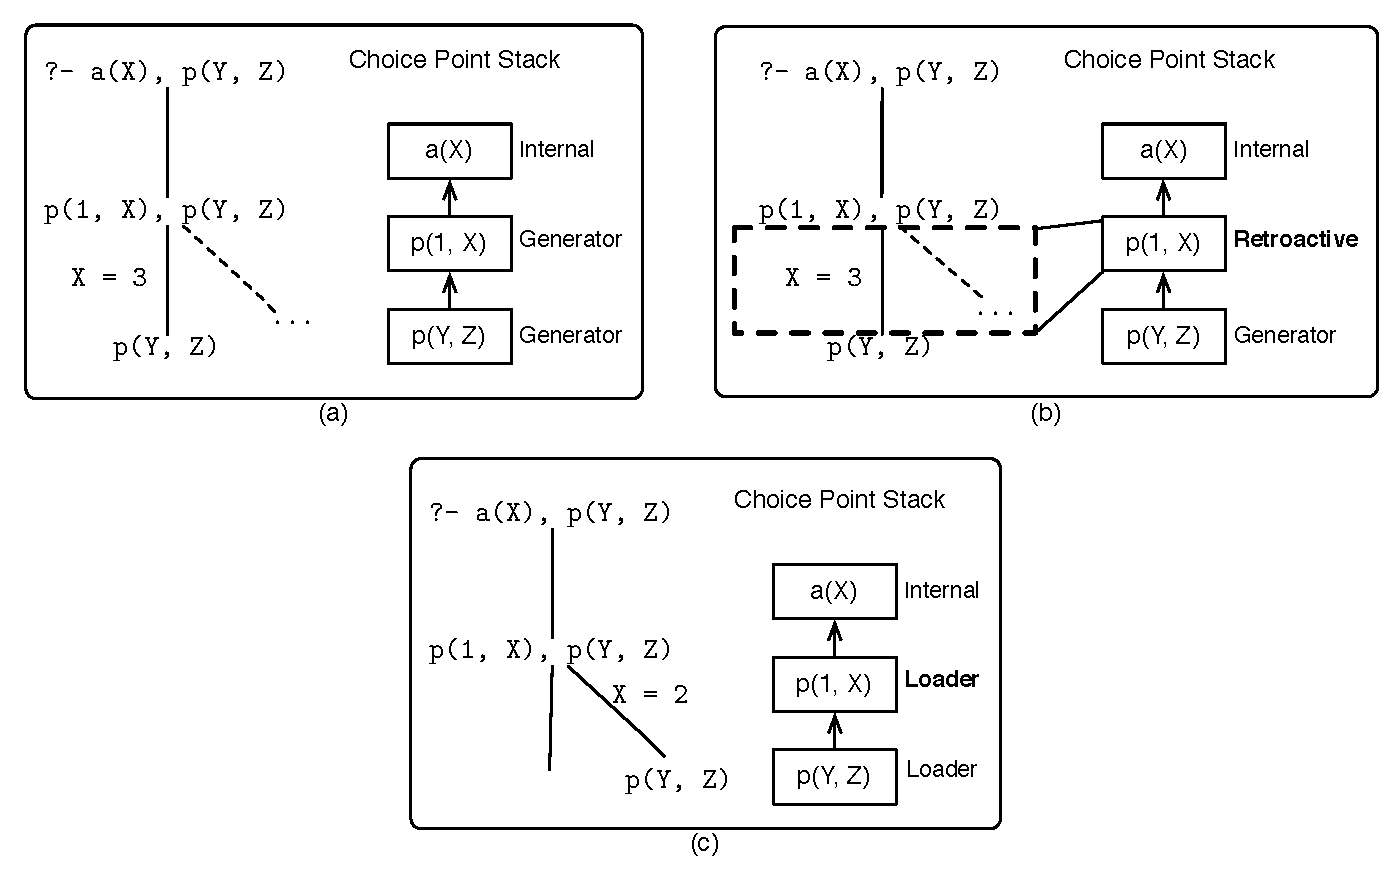
\includegraphics[scale=0.6]{pruning_example1.pdf}
  \caption{Evaluating `\texttt{a(X),~p(Y,Z)}' using retroactive tabling.}
  \label{fig:retro_eval1}
\end{figure}

The previous example has illustrated one special type of pruning called \textit{external pruning}.
External pruning occurs when the subsuming subgoal $G'$ is an \textit{external subgoal} to the evaluation
of the subsumed subgoal $G$. Another type of pruning is called \textit{internal pruning} and happens
when $G'$ is an \textit{internal subgoal} to the evaluation of $G$, that is, $G'$ is called
during the resolution of $G$. Although these two basic types of pruning can derive any other
situation, they both generate the same issues related to evaluation pruning. These issues will be explored
in detail in the next section.

\section{Pruning: Rules and Issues}

When pruning parts of the computation, we must know the areas of the local stack
that contain the choice points to prune. Given the nature of the tabling evaluation, choice points not
directly related to the pruned subgoal can get mixed with other choice points. This happens when a branch
containing external choice points has been suspended, but after backtracking to internal choice points we
execute a subsuming subgoal. Therefore, we must have a mechanism that can tell us if a certain choice
point is internal to a subgoal, from a range of choice points that can potentially be from
the pruned subgoal.

For this, we construct a dependency tree of subgoals and dependency frames by storing in a field
called \textbf{top\_gen} a pointer to the top tabled subgoal. Thus, by traversing this field we know
what subgoals the target subgoal or consumer is internal to.

When pruning execution branches, issues arise mostly when the computation of the subsumed subgoal involves
consumer and/or generators nodes. The next example programs will illustrate these issues.

Consider the program in Figure~\ref{fig:retro_program2} that mixes tabled predicates using retroactive
and variant-based tabled predicates.
For this program, we will use the query goal `\texttt{a(X,Y),~p(Z,W)}'.

\begin{figure}[ht]
\begin{Verbatim}
:- use_variant_tabling [a/2, b/1].
:- use_retroactive_tabling p/2.

a(X, Y) :- p(1, X), b(Y).
a(3, 4).

b(1).
b(2).

p(1, X) :- a(_, X).
p(1, X) :- b(X).
\end{Verbatim}
\caption{Example program using retroactive tabling with variant tabling.}
\label{fig:retro_program2}
\end{figure}

Initially, evaluation calls \texttt{a(X,Y)} and a new generator node is stored. Next, the retroactive subgoal
\texttt{p(1,X)} is called and creates a new generator node, because no subsuming subgoal is found.
The first clause of \texttt{p/2} executes \texttt{a(\_,X)}, which is a consumer of \texttt{a(X,Y)}, but, as
no answers are available to consume, execution suspends this node and backtracks to try to second clause
of \texttt{p/2}. Here, \texttt{b(X)} is called for the first time, creating a new generator choice point.
An answer for \texttt{b(X)} is generated, \texttt{\{X~=~1\}}, and by forward execution it is also an answer
for \texttt{p(1,X)}. Next, \texttt{b(Y)} is called, creating a new consumer node that consumes the answer
\texttt{\{X~=~1\}} and by forward execution, the first answer for \texttt{a(X,Y)}, \texttt{\{X~=~1,~Y~=~1\}},
is generated.

\begin{figure}[ht]
  \centering
    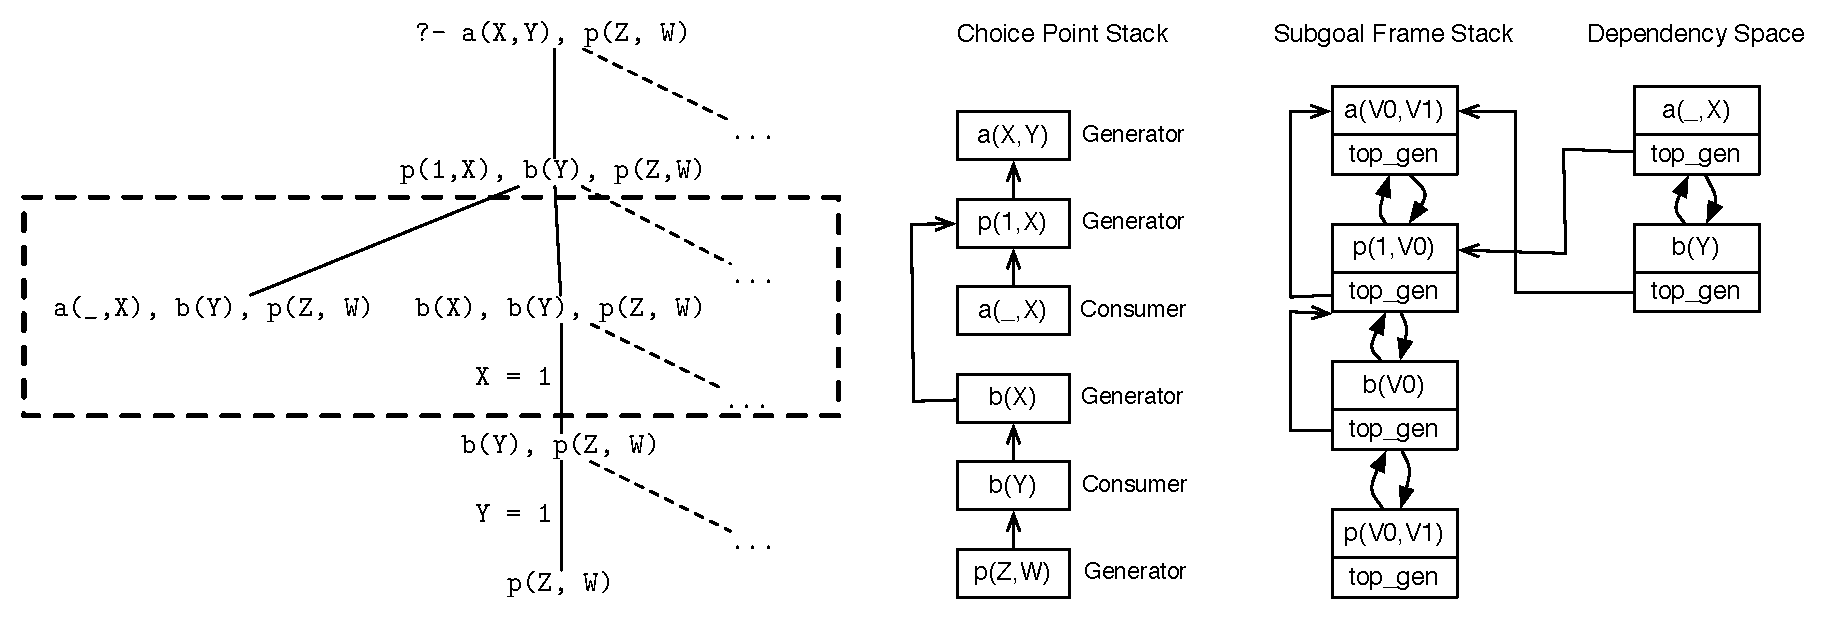
\includegraphics[scale=0.5]{retro_example2.pdf}
  \caption{Evaluating `\texttt{a(X,Y),~p(Z,W)}' using retroactive tabling.}
  \label{fig:retro_eval2}
\end{figure}

Next, subgoal \texttt{p(Z,W)} is called, which subsumes \texttt{p(1,X)} and the evaluation of this subgoal
must be pruned (Figure~\ref{fig:retro_eval2}). As \texttt{p(Z,W)} is external to \texttt{p(1,X)} we have
a case of external pruning. Please notice that \texttt{p(1,X)} now includes various choice
points involved in its computation, namely \texttt{a(\_,X)} and \texttt{b(X)}.

The consumer node associated with the subgoal \texttt{a(\_,X)} must leave the computation and no longer
participates in answer resolution, thus its dependency frame is removed from the dependency space.

Pruning the generator node associated with the subgoal \texttt{b(X)} is a more tricky case. Notice that
the consumer \texttt{b(Y)} depends on this subgoal to consume new answers, thus by removing the generator node
the consumer will become an \textit{orphaned consumer} and the computation will not complete properly.
Therefore, we mark the subgoal \texttt{b(X)} as \textit{pruned} and turn the consumer node of \texttt{b(Y)}
into a retroactive node. Finally, the \textit{previous choice point} field of the choice point associated
with \texttt{b(Y)} must now point to \texttt{p(1,X)}, because we must prevent the evaluation to step into
pruned branches by means of backtracking. The choice point of \texttt{b(Y)} is called a
\textit{frontier choice point}. Figure \ref{fig:retro_eval3} shows the state of the computation after pruning.

\begin{figure}[ht]
  \centering
    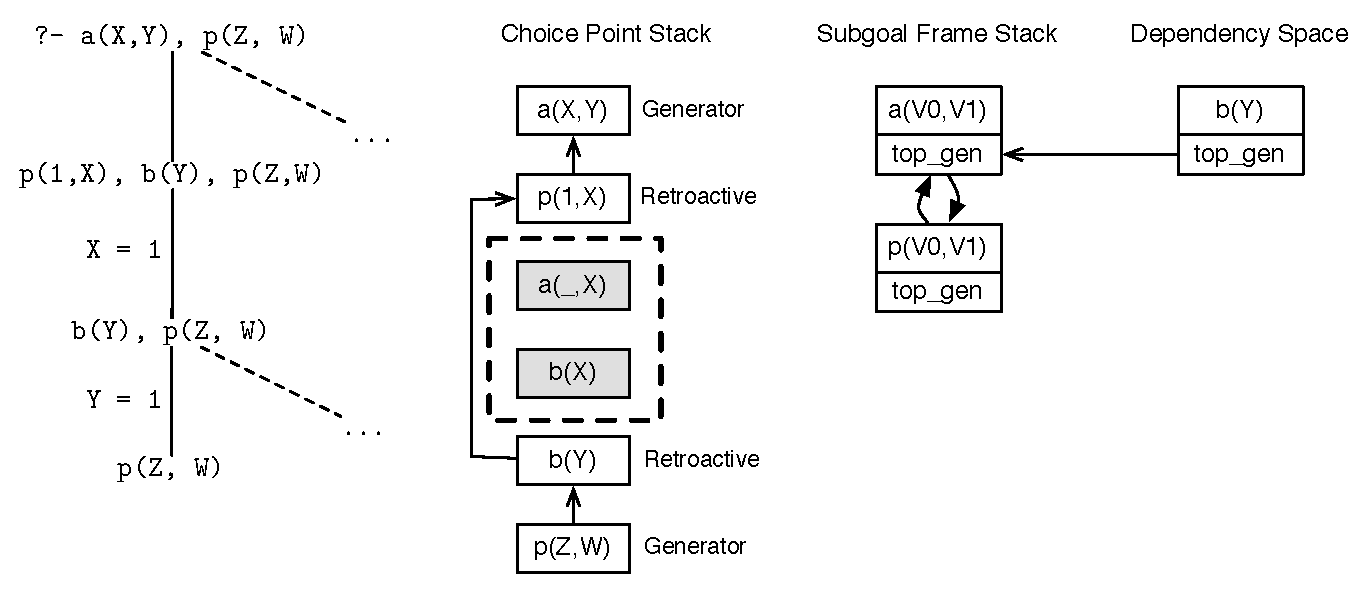
\includegraphics[scale=0.5]{retro_example3.pdf}
  \caption{After external pruning over choice points belonging to the subsumed subgoal.}
  \label{fig:retro_eval3}
\end{figure}

Next, the subgoal \texttt{p(Z,W)} starts to execute the first clause of \texttt{p/2} and creates
a new consumer for \texttt{a(\_,X)}, that will consume one answer. By forward execution, an answer
for \texttt{p(Z,W)}, \texttt{\{Z~=~1,~W~=~1\}}, is generated. By means of backtracking, the second
clause of \texttt{p/2} is executed and \texttt{b(Y)} is called. As the subgoal \texttt{b(Y)} is a pruned subgoal,
we first load the answers already generated for this subgoal and then execute the clauses of \texttt{b/1}.
After \texttt{b(Y)} generates all the answers, it completes successfully and execution backtracks to
\texttt{p(Z,W)}, to attempt completion of this subgoal. As the leader node is currently \texttt{a(X,Y)},
completion fails.

We backtrack to the retroactive node \texttt{b(Y)} in order to do retroactive resolution. Evaluation
notices that the subgoal has already completed, thus the retroactive node is transformed into a loader node
to consume all answers that were not consumed. By forward execution, a new consumer for \texttt{p(Z,W)} is
created that will generate more answers for the query goal. Once \texttt{b(Y)} does not have more answers
to consume, execution backtracks to the retroactive node of \texttt{p(1,X)}. Here, we note that
the generator subgoal, \texttt{p(Z,W)} has still not completed and this retroactive node must be turned
into a consumer node, which amounts to create a new dependency frame that is added into the dependency space,
in order to participate in the resolution process.

After \texttt{p(1,X)} executes the answer resolution
operation, evaluation backtracks to \texttt{a(X,Y)} that will execute the second clause of \texttt{a/2}.
Once \texttt{a(X,Y)} executes the completion operation and each each consumer has consumed its answers,
the subgoal completes and evaluation is finished.

\subsection{Pruning Actions}

The previous example has illustrated the different actions that must be applied to each choice point that
makes part of the computation of the subsumed subgoal. This action is dependent on the choice point
type and is summarized in the next subsections.

\subsubsection{Interior Nodes}

Interior nodes are related to normal Prolog execution and can be easily pruned
by ignoring them altogether. This approach, while simple, suffers from the problem of \textit{trapped
choice points}. This problem also affects the normal execution of delaying based tabling engines like
YapTab and SLG-WAM, where choice points under consumers are frozen and remain until completion.
The CHAT approach to tabling solves this problem by removing trapped choice points \cite{Demoen-99b}.
Another solution would involve modifications to the WAM garbage collector to collect unused space on
the choice point stack.

\subsubsection{Internal Consumers}   
   
Internal consumers must be explicitly pruned by removing the associated
dependency frame from the dependency space. This prevents the resolution process to reactivate pruned
branches. In the previous example, \texttt{a(\_,X)} was an internal consumer.

\begin{figure}[ht]
\begin{Verbatim}
abolish_dependency_frames(specific_sg, min, max) {
   top = TOP_DEP_FR
   
   while (top != NULL and younger_than(cons_cp(top), max))
     top = next(depfr)
     
   while (top != NULL and younger_than(cons_cp(top), min))
      depfr = top
      top = next(depfr)

      if (is_internal_depfr(specific_sg, depfr, min))
         remove_from_stack(depfr)
         free(dep_fr)
}
\end{Verbatim}
\caption{Pseudo-code for procedure \texttt{abolish\_dependency\_frames}.}
\label{fig:abolish_dependency_frames}
\end{figure}
   
Figure~\ref{fig:abolish_dependency_frames} shows the procedure that abolishes internal dependency frames.
The arguments are: \texttt{specific\_sg}, the subsumed subgoal to prune; \texttt{min}, the first choice
point address from the range of choice points to selectively prune; and \texttt{max}, the last choice point
from the pruned range. First, we ignore dependency frames younger than the \texttt{max} choice point.
Next, we iterate the dependency frames inside the range and check if they are internal to the choice point;
if they are, we remove them from the dependency space.

\subsubsection{Internal Generators}

For internal generators we must remove its corresponding subgoal frame
from the subgoal frames stack and alter its state to pruned. Generally, when pruning internal generators, we
have two situations: (1) the generator does not have consumers that are external to the computation of the
subsumed subgoal; or (2) the generator has external consumers. The former situation does not introduce any
problem, but the latter origins orphaned consumers. In our previous example, the consumer node for \texttt{b(Y)} is
an orphaned consumer.

Usually, a pruned generator is called again during the evaluation of the subsuming subgoal, and before
the computation reaches any of the orphaned consumers. Once reactivated, the subgoal frame for the pruned
generator is pushed again into the top of the subgoal frame stack and its state is altered to
\textit{evaluating}. Then, the new generator node starts by consuming the previously generated answers
and only then executes the program clauses.

\begin{figure}[ht]
\begin{Verbatim}
abolish_subgoal_frames(specific_sg, min, max) {
   top = prev(specific_sg)

   remove_subgoal_from_stack(specific_sg)
   
   while (top != NULL and !younger(generator_cp(top), max))
      sg_fr = top
      top = prev(sg_fr)

      if (is_internal_subgoal_frame(specific_sg, sg_fr, min))
         sg_cp = generator_cp(sg_fr)
         
         remove_subgoal_from_stack(sg_fr)
         
         if (type(sg_fr) == VARIANT or type(sg_fr) == RETROACTIVE)
            if (has_external_consumers(sg_fr))
               update_external_consumers(specific_sg, sg_fr, sg_cp, max)
               state(sg_fr) = pruned
            else
               free(sg_fr)
         else if (type(sg_fr) == SUBSUMPTIVE)
            if (has_subsumed_consumers(sg_fr))
               transform_external_subsumed_consumers(specific_sg, sg_fr, sg_cp, max,
                  has_variant_consumers(sg_fr))
            
            if (has_variant_consumers(sg_fr))
               update_external_consumers(specific_sg, sg_fr, sg_cp, max)
               state(sg_fr) = pruned
               
            if (has_no_consumers(sg_fr))
               free(sg_fr)
}
\end{Verbatim}
\caption{Pseudo-code for procedure \texttt{abolish\_subgoal\_frames}.}
\label{fig:abolish_subgoal_frames}
\end{figure}

Figure~\ref{fig:abolish_subgoal_frames} shows the procedure \texttt{abolish\_subgoal\_frames} that is
responsible in abolishing internal generators. For variant and retroactive-based tabled subgoals we remove
the subgoal frame from the stack (using \texttt{remove\_subgoal\_from\_stack}) and then check if the
subgoal has external consumers. If those consumers are found, they are turned into retroactive nodes
by the procedure \texttt{update\_external\_consumers}.

Our system is also able to mix tabled subgoals using traditional call subsumption with retroactive-based tabling.
For this case we distinguish between variant consumers (identical consumers by variable renaming) and
subsumed consumers (proper subsumed consumers).
If the subgoal has no external variant consumers, we remove the subgoal frame from the system and
its path from the subgoal trie, which means that external subsumed consumers are turned into generators as
the generator has been deleted. When we have external variant consumers, the pruned subgoal changes its state
to \textit{pruned} in order to be reactivated later or by an orphaned consumer.

A tricky situation happens when an orphaned variant consumer is pruned by another subgoal and orphaned
subsumed consumers are left in a situation where the generator subgoal will not be reactivated. In this case,
we check for situations where the subsumptive subgoal has no more variant consumers and we change its state
to \textit{dead}. Later on, when a subsumed consumer is reactivated by means of retroactive resolution, we
verify if the generator is \textit{dead}. If this is the case, we simply convert the subgoal frame to a
subsuming subgoal frame and turn the retroactive node into a generator. This also involves modifications
to the answer template, which must be transformed into a generator answer template (with only variables).

For an example using subsumptive subgoals, consider the program in Figure~\ref{fig:retro_sub} and
the query goal `\texttt{p(1,A),~t(1,2,B),~b(1,C),~p(D,E),~b(F,G)}'.

\begin{figure}[ht]
\begin{Verbatim}
:- use_retroactive_tabling [b/2, p/2].
:- use_subsumptive_tabling t/3.

p(X, 55) :- t(X, A, B).
p(1, 5).
p(10, 10).

b(X, 20) :- t(X, A, B).
b(3, 1).

t(1, 2, 3).
t(1, 2, 5).
t(3, 10, 20).
\end{Verbatim}
\caption{Example program using retroactive tabling with subsumptive tabling.}
\label{fig:retro_sub}
\end{figure}

The first goal \texttt{p(1,A)}
creates a new generator node and calls \texttt{t(1,A,B)}, which is considered a subsumptive generator subgoal.
By forward execution we call the subgoal \texttt{t(1,2,B)}, which will create a consumer node that subsumes
the subgoal \texttt{t(1,A,B)}. Next, we make another retroactive call (\texttt{b(1,C)}) that creates
another generator and calls \texttt{t(1,A,B)}, which is a variant consumer of the initial the subsumptive generator.
Finally, we call \texttt{p(D,E)} and \texttt{p(1,A)} must be pruned (Figure~\ref{fig:retro_sub1}).

\begin{figure}[ht]
  \centering
    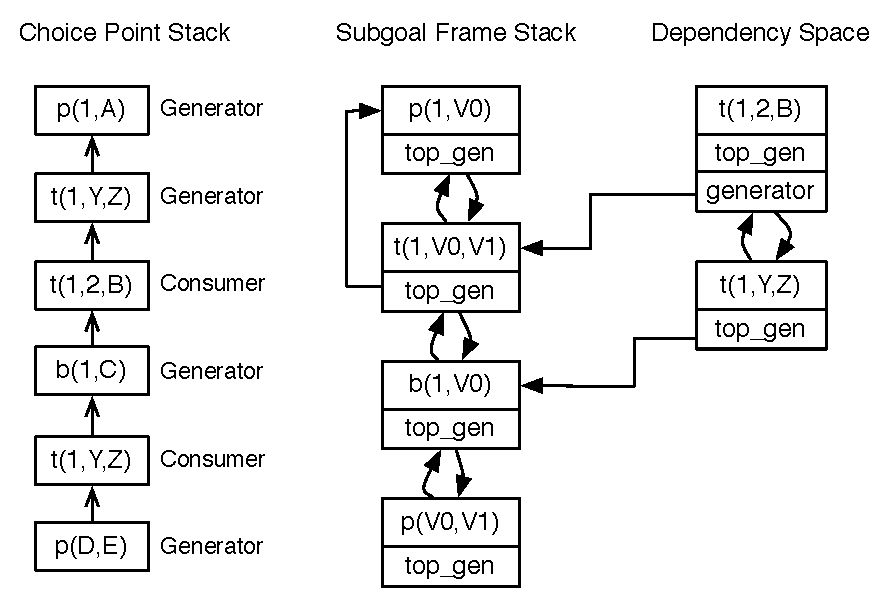
\includegraphics[scale=0.5]{retro_sub1.pdf}
  \caption{Evaluation before pruning subsumptive subgoals using the subgoal \texttt{p(C,D)}.}
  \label{fig:retro_sub1}
\end{figure}

The generator \texttt{t(1,A,B)} is internal to \texttt{p(1,A)} and has two external consumers: one variant
and one subsumed consumer,\texttt{t(1,2,B)}. Here, we modify the state of subsumptive subgoal to \textit{pruned}
and turn each external consumer node into retroactive nodes. We are hoping that \texttt{t(1,A,B)} will be
reactivated and \texttt{t(1,2,B)} will continue to consume from its generator. Figure~\ref{fig:retro_sub2}
shows the state of computation after pruning.

\begin{figure}[ht]
  \centering
    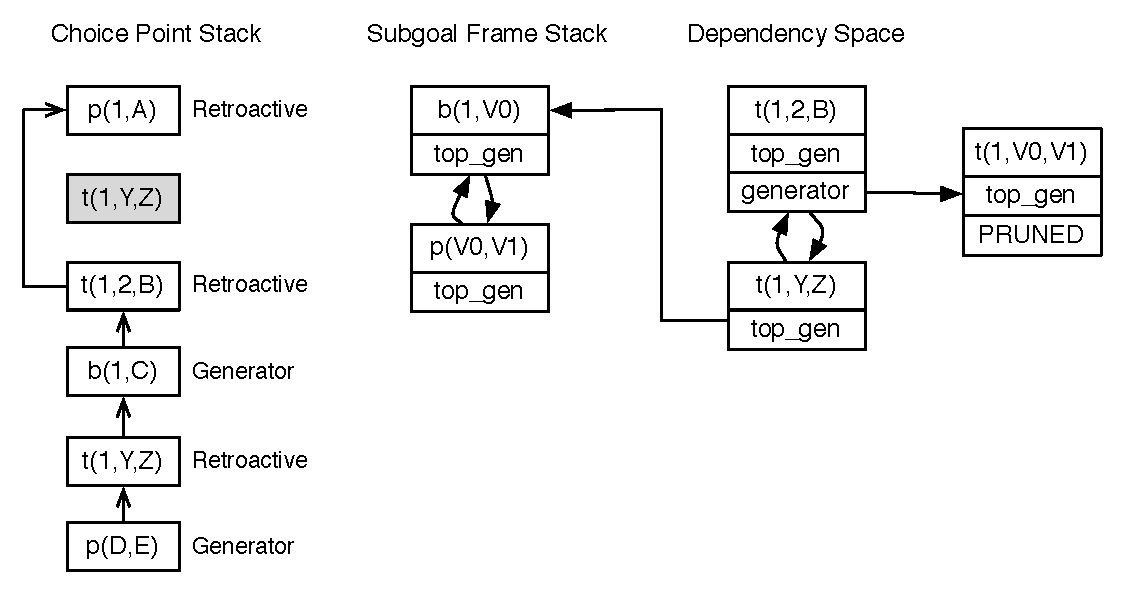
\includegraphics[scale=0.5]{retro_sub2.pdf}
  \caption{Evaluation after pruning subsumptive subgoals using the subgoal \texttt{p(C,D)}.}
  \label{fig:retro_sub2}
\end{figure}

Next, evaluation of \texttt{p(C,D)} generates a call to the subsumptive subgoal \texttt{t(X,A,B)}, which
is a generator subgoal. By forward execution, we call \texttt{b(F,G)} which subsumes \texttt{b(1,C)} and triggers
a new external pruning operation. The computation of \texttt{b(1,C)} contains the internal consumer
\texttt{t(1,A,B)} that is currently associated with a retroactive node. We delete this consumer from the
dependency space and as \texttt{t(1,A,B)} has no more variant consumers that can reactivate this subgoal,
we update its state to \textit{dead}, in order to inform retroactive nodes that dependent on it that the generator
will no longer produce answers (in this example, \texttt{t(1,2,B)}). The result of pruning is shown in
Figure ~\ref{fig:retro_sub3}.

\begin{figure}[ht]
  \centering
    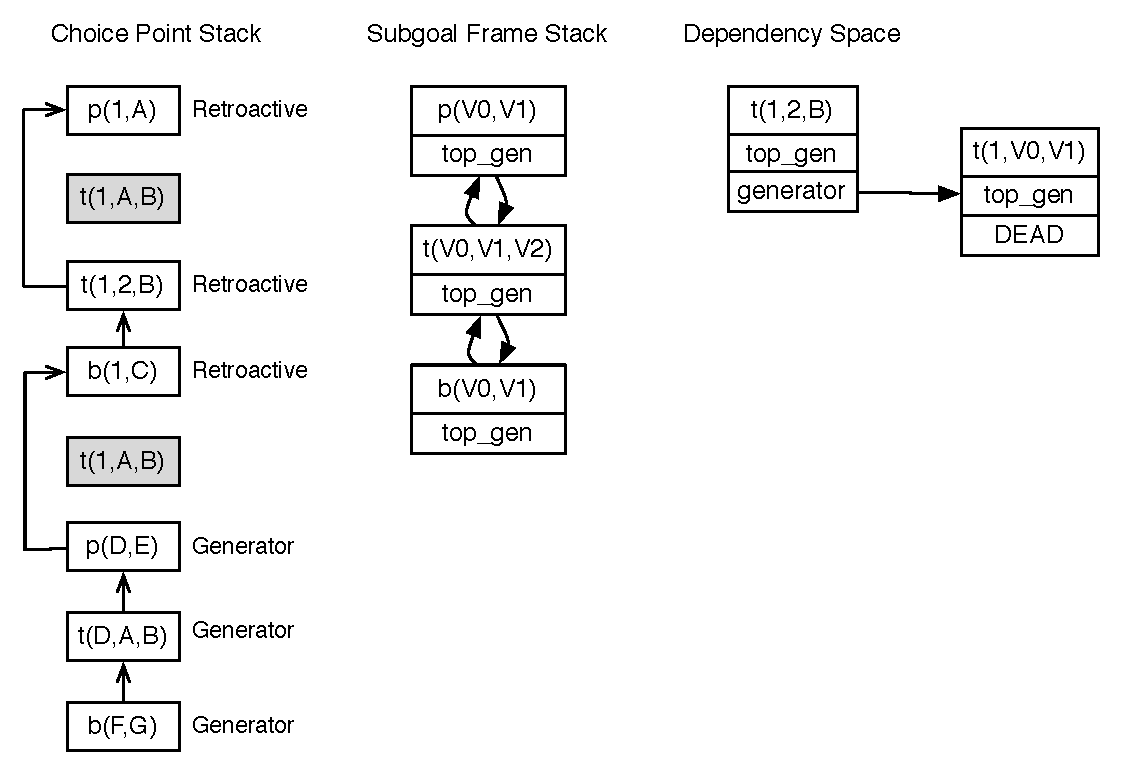
\includegraphics[scale=0.5]{retro_sub3.pdf}
  \caption{Evaluation after pruning subsumptive subgoals using the subgoal \texttt{b(F,G)}.}
  \label{fig:retro_sub3}
\end{figure}

After the subgoals \texttt{b(F,G)}, \texttt{t(X,A,B)} and \texttt{p(D,E)} complete, we backtrack to
the retroactive node \texttt{b(1,C)}. This node is transformed into a loader node as the generator
subgoal has already completed. After the answers have been exhausted, we backtrack to the retroactive
node \texttt{t(1,2,B)}. As the current generator subgoal is \textit{dead} we transform the consumer subgoal
frame into a generator subgoal frame and the retroactive node is transformed into a generator node, because
the subgoal must now generate its own answers. In order for this to work, the answer template is transformed
from \texttt{\{2,~2,~B\}} to \texttt{\{1,~B\}}. Figure \ref{fig:retro_sub4} shows the state of the computation
after this transformation.

\begin{figure}[ht]
  \centering
    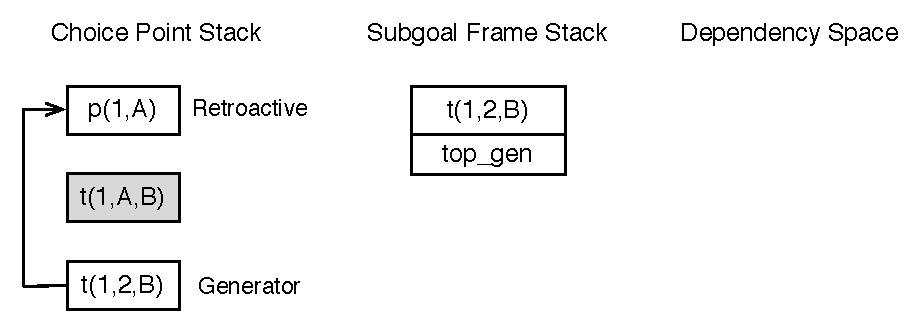
\includegraphics[scale=0.5]{retro_sub4.pdf}
  \caption{Evaluation after transforming the subsumed consumer \texttt{t(1,2,B)} in a subsumptive generator.}
  \label{fig:retro_sub4}
\end{figure}

\subsection{Orphaned Consumers}

An orphaned consumer is an external consumer that loses its generator after a pruning operation.
As we have seen, we transform each orphaned consumer node into a retroactive node.
When an orphaned consumer node is reached by means of backtracking it will be transformed into either:
(1) a loader node, if the pruned generator was reactivated and has completed; (2) a consumer node,
if the pruned generator was reactivated but has not completed yet, which means that below the new pruned subgoal
choice point there is a dependency on a upper generator node, thus this new consumer will participate
in the completion operation as usual; or (3) a generator node,
if the pruned generator was not reactivated until then. This latter situation only occurs with
variant or subsumptive tabling. With retroactive tabling, the execution of the subsuming subgoal
will call the same or a more general subgoal, and this subgoal will update the \textbf{producer} field
of any subsumed subgoal frame, including orphaned consumers.

By default, orphaned consumers always keep their frames on the dependency frame stack. The frame is only
removed if the retroactive node turns into a loader or generator node. If the retroactive node turns again
into a consumer node, lazy removal of dependency frames allows us to avoid removing and allocating a new
frame and the potentially expensive operation of inserting it on the dependency frame stack in the
correct order (ordered by choice point address).

\subsection{Lost Consumers}

While it is usually possible to transform each retroactive node into the correct type of node by means
of backtracking or answer resolution, there are some cases where this is not possible. This happens to
external consumers turned into retroactive nodes and we call them \textit{lost consumers}.

For an example, consider the program in Figure~\ref{fig:retro_lost_consumer_code} and the query goal
`\texttt{a(X,Y)}'.

\begin{figure}[ht]
\begin{Verbatim}
:- use_variant_tabling [a/2, b/2].
:- use_retroactive_tabling p/2.

a(X, 0) :- p(1, X).
a(0, Y) :- b(1, Y).
a(X, Y) :- p(X, Y).

b(1, Y) :- a(_, Y).
b(2, 1).

p(X, Y) :- b(X, Y).
\end{Verbatim}
\caption{Example program with a lost consumer.}
\label{fig:retro_lost_consumer_code}
\end{figure}

Evaluation starts by storing a generator node for \texttt{a(X,Y)} and then calling
the retroactive subgoal \texttt{p(1,X)}.
Next, the subgoal \texttt{b(1,X)} is called, creating a new
generator node; consequently \texttt{b(1,X)} calls subgoal \texttt{a(\_,Y)} that is a variant of the
first called subgoal and thus a consumer node is stored. As no answers are available to consume,
evaluation suspends and then backtracks to the second clause of \texttt{b/2}, but it does not
unify with \texttt{b(1,X)}. By backtracking, we attempt the second clause of \texttt{a/2}, which
originates a call to \texttt{b(1,Y)}. This is a variant call of \texttt{b(1,X)} and a new consumer is
created. This node must be suspended as no answers are available.

Through backtracking, we execute the second clause of \texttt{a/2} and the retroactive subgoal \texttt{p(X,Y)}
is called. As this subgoal subsumes \texttt{p(1,X)} we must prune the evaluation of \texttt{p(1,X)}.
The internal generator \texttt{b(1,X)} is pruned, leaving an orphaned consumer, \texttt{b(1,Y)}. The internal
consumer \texttt{a(\_,X)} is simply thrown away. Note that here, we do not have a frontier choice point,
because the subsumed subgoal appears outside the branch of the subsuming subgoal. This is safe, because
the branch including the subsumed subgoal will only be resumed on consumers during completion and thus
no backtracking to previous choice points will occur as they were fully explored before.

After \texttt{p(X,Y)} is fully explored, the following answers are generated for the subgoal \texttt{a(X,Y)}:
\texttt{\{X~=~1,~Y\}} and \texttt{\{X~=~2,~Y~=~1\}}. Then, we attempt completion at the leader node,
\texttt{a(X,Y)} (Figure~\ref{fig:retro_lost_consumer}). At this point, \texttt{b(1,Y)} still remains
a retroactive node and it is clear that it must be resumed in order to be reactivated as a generator,
and consequently, generate more answers to \texttt{a(X,Y)}, namely \texttt{\{X~=~0,~Y~=~1\}} and
\texttt{\{X~=~0,~Y~=~1\}}. Note that \texttt{b(1,Y)} is not a real consumer and thus can not participate
in the completion operation before retroactive resolution is applied. Therefore, to ensure that all
retroactive nodes are resumed, the completion is extended to, while traversing the dependency space
checking for new answers, also \textit{check for retroactive nodes}, and resume the corresponding
consumer node in both cases. In the example, \texttt{b(1,Y)} is resumed and transformed into a
generator node, thus allowing the computation to finish correctly.

\begin{figure}[ht]
  \centering
    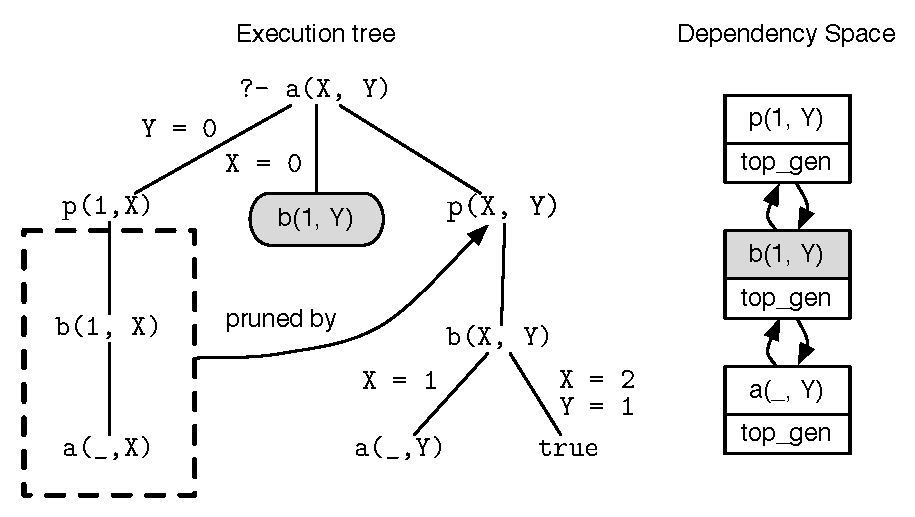
\includegraphics[scale=0.6]{retro_lost_consumer.pdf}
  \caption{Lost consumer \texttt{b(1,Y)} after an external pruning.}
  \label{fig:retro_lost_consumer}
\end{figure}

\subsection{Pseudo-Completion}

When the subsumed subgoal $G$ is pruned when it is a leader node for some consumers, the completion operation
will not be run at node $G$ because $G$ is now a retroactive node and we will not be able to resume
consumers that do not have been fully explored by other leader nodes. Therefore, we must ensure
that every consumer is resumed in order to fully explore every evaluation branch.

Consider the query goal `\texttt{p(1,A,B),~p(1,3,C),~p(D,E,F)}' and the program in Figure~\ref{fig:retro_ignored_consumer}. After the call to \texttt{p(1,A,B)} succeeds with the
answer \texttt{\{A~=~2,~B~=~3\}}, subgoal \texttt{p(1,3,C)} is called and a new consumer of
\texttt{p(A,B,C)} is created (consumer $C1$). As no answers are available to consume, execution
backtracks to \texttt{p(1,A,B)} and a second answer is generated, \texttt{\{A~=~3,~B~=~2\}}. Next,
subgoal \texttt{p(1,3,C)} is called again and a new consumer is generated (consumer $C2$).
This consumers consumes the answer \texttt{\{C~=~2\}} and execution proceeds. 

\begin{figure}[ht]
\begin{Verbatim}
:- use_retroactive_tabling p/2.

p(1, 2, 3).
p(1, 3, 2).
\end{Verbatim}
\caption{Example program for pseudo-completion.}
\label{fig:retro_ignored_consumer}
\end{figure}

Subgoal \texttt{p(D,E,F)} is called and must prune the evaluation of \texttt{p(1,A,B)} 
(Figure~\ref{fig:retro_pseudo_completion1}). Both subgoal frames, \texttt{p(1,A,B)} and \texttt{p(1,3,C)}
are turned into consumer subgoal frames and their \textbf{producer} field is set to the subgoal
frame of \texttt{p(D,E,F)}.

\begin{figure}[ht]
  \centering
    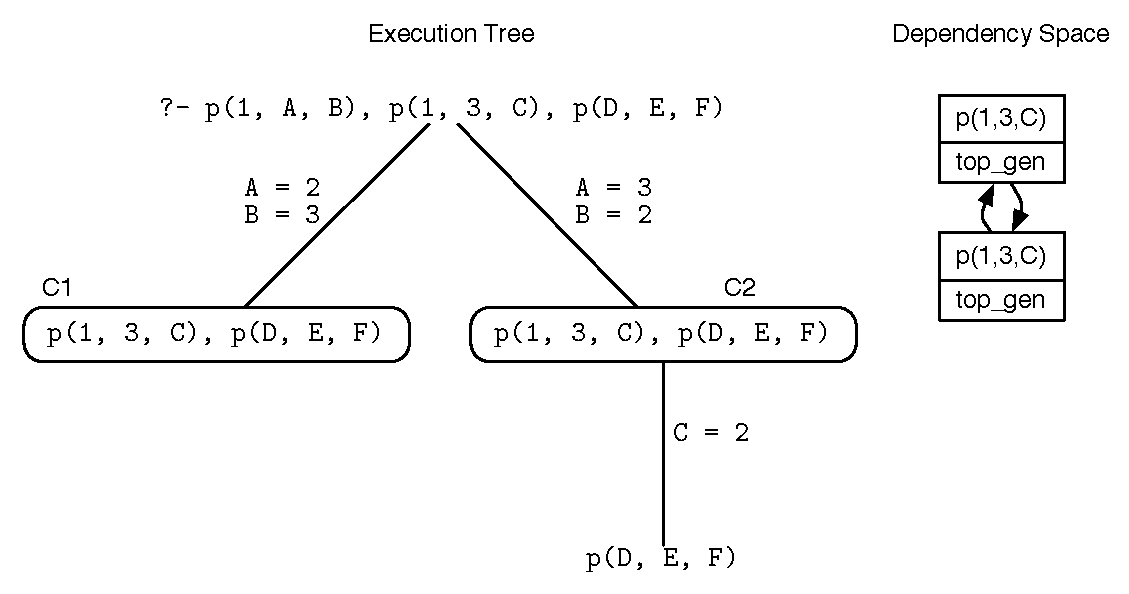
\includegraphics[scale=0.6]{retro_pseudo_completion1.pdf}
  \caption{Query goal `\texttt{p(1,A,B),~p(1,3,C),~p(D,E,F)}' before pruning.}
  \label{fig:retro_pseudo_completion1}
\end{figure}

After \texttt{p(D,E,F)} completes, execution backtracks to retroactive node $C2$ that is transformed
in a loader node by retroactive resolution. After all answers are loaded, execution backtracks to
the retroactive node of \texttt{p(1,A,B)}. If we transform the retroactive node into a loader node and
then load all the answers relevant to this node we might lose the consumer $C1$, because there is no
other way to reach that node.

Notice that when consumer $C1$ has been created its leader node was
\texttt{p(1,A,B)}. Hence, before loading all answers, we act as a \textit{pseudo-leader} (since no upper
dependencies exist) and we look for younger retroactive nodes with unconsumed answers on the dependency
frame stack. When we find node $C1$, we set the field \textbf{backchain\_cp} of the target dependency
frame to the choice point of the pseudo-leader and computation is resumed at $C1$
(Figure \ref{fig:retro_pseudo_completion2}).

After $C1$ is solved
through retroactive resolution, it loads all its answers and, instead of backtracking, jumps to the choice
point saved in the \textbf{backchain\_cp} field, thus allowing the pseudo-leader to resume other retroactive
nodes. The reason to use the \textbf{backchain\_cp} field instead of backtracking, is because any choice
point between the pseudo-leader and the target consumer as been fully exploited, thus we must jump explicitly
between nodes. The process of resuming consumers through a pseudo-leader is called \textit{pseudo-completion}.

\begin{figure}[ht]
  \centering
    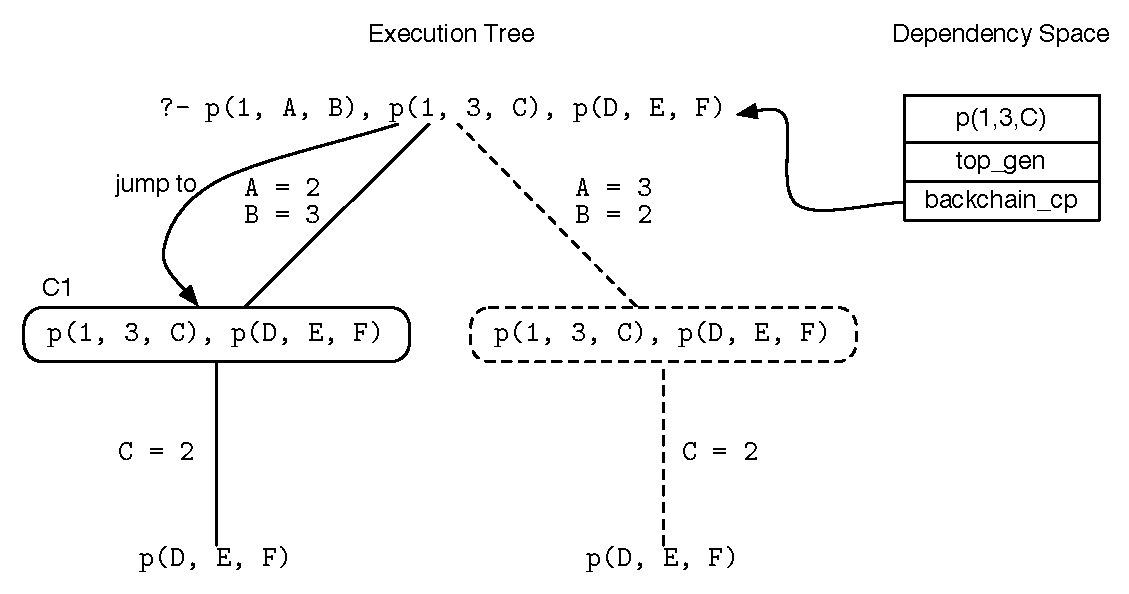
\includegraphics[scale=0.6]{retro_pseudo_completion2.pdf}
  \caption{Executing a pseudo-completion.}
  \label{fig:retro_pseudo_completion2}
\end{figure}

\subsection{Leader Re-Computation}

Each dependency frame contains the value of the leader node during the creation of the consumer node.
External consumers can reference as a leader either: (1) a pruned generator choice point; or (2) a
generator that appeared before the execution of the subsumed subgoal. In the second case we keep
the dependency frame unmodified. In the first case, we update the leader choice point (\textbf{leader\_cp})
field to the consumer node itself.

The reason we update the \textbf{leader\_cp} field is to avoid the leader computation algorithm to compute
a leader that simply does not exist, making completion impossible.
For an example describing this problem, consider the program in Figure~\ref{fig:retro_leader_program}
and the query goal `\texttt{p(1,A),~a(B,C),~a(1,D),~p(E,F)}'.

\begin{figure}[ht]
\begin{Verbatim}
:- use_retroactive_tabling p/2.
:- use_variant_tabling p/2.

a(1, 3).
a(1, 2).
a(2, 4).

p(X, Y) :- a(X, Y).
\end{Verbatim}
\caption{Example program demonstrating the leader re-computation problem.}
\label{fig:retro_leader_program}
\end{figure}

During the evaluation of the subgoal \texttt{p(1,A)}, a generator node
for \texttt{a(1,Y)} is created. Next, a new generator is allocated for \texttt{a(B,C)},
followed by the consumer node \texttt{a(1,D)}. When \texttt{p(E,F)} is called to
prune \texttt{p(1,A)} (Figure~\ref{fig:retro_leader_recomputation}), the generator \texttt{a(1,Y)}
is pruned and the \textbf{leader\_cp}
field of the consumer \texttt{a(1,D)} still points to \texttt{a(1,Y)}.
During execution of \texttt{p(E,F)} a new consumer is allocated for \texttt{a(X,Y)} that
decides its leader should be the pruned \texttt{a(1,X)} generator, because between
the generator and consumer nodes, the \texttt{a(1,D)} consumer has an older leader.

\begin{figure}[ht]
  \centering
    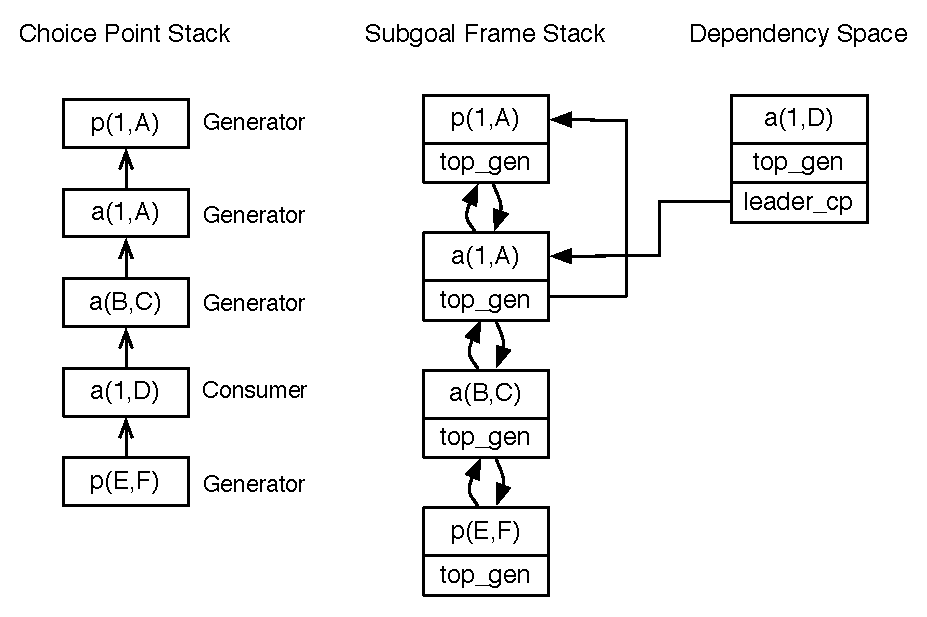
\includegraphics[scale=0.6]{retro_leader_recomputation.pdf}
  \caption{Before pruning the subsumed subgoal.}
  \label{fig:retro_leader_recomputation}
\end{figure}

Finally, execution proceeds and completion is attempted at the subgoal \texttt{p(E,F)}.
Because this is not the leader node, we backtrack to \texttt{a(1,D)} that is transformed
into a generator and then completes. Next, we backtrack to \texttt{a(B,C)} to try other
alternatives of \texttt{a/2} and then completion is attempted, but without success because
the leader node is the pruned generator \texttt{a(1,Y)}. It is then impossible to complete
the evaluation because the leader node is never reached.

By our delineated rules, the \texttt{leader\_cp} of the consumer \texttt{a(1,D)} would have been
modified to itself, thus making the generator \texttt{a(B,C)} the leader of the computation.
Notice that the consumer node, \texttt{a(X,Y)} created during the evaluation of \texttt{p(E,F)} would
consider that its leader was \texttt{a(B,C)}. Figure~\ref{fig:retro_leader_recomputation2} shows the
state of computation at that point.

\begin{figure}[ht]
  \centering
    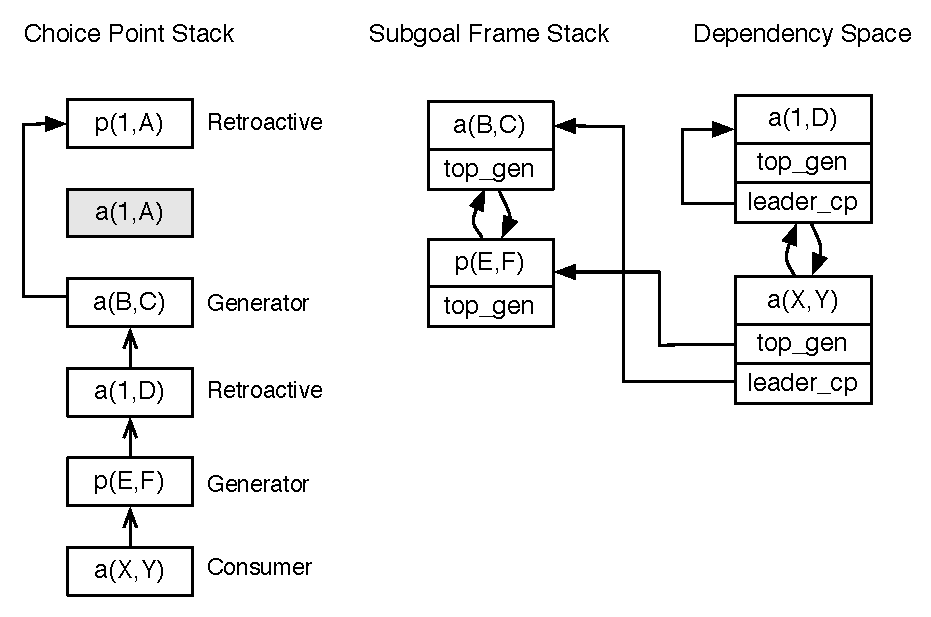
\includegraphics[scale=0.6]{retro_leader_recomputation2.pdf}
  \caption{Updated \textbf{leader\_cp} fields.}
  \label{fig:retro_leader_recomputation2}
\end{figure}

\section{Internal Pruning}

Although all the previous examples used external pruning, both external and internal pruning
suffer from the issues previously described. This section explores internal pruning
and its differences in relation to external pruning.

Internal pruning occurs when the subsuming subgoal $S$ is internal to the evaluation of the
subsumed subgoal $R$. In this type of pruning we want to keep one part of $R$ running, the one
that computes $S$, hence we are able to compute all answers of $R$ just by computing $R$.

Our approach involves computing $S$ using local scheduling \cite{Freire-96}, but without returning
answers to the environment of $R$, as it has been pruned. Instead, we jump directly to the
choice point of $R$, which was transformed into a retroactive node, and resume the computation there
in order to consume the matching answers found by $S$. When resuming the retroactive node for $R$, it
can become either: (1) a loader node, if $S$ has completed; or (2) a consumer node, if $S$ has not
completed because it is not the leader node, i.e., the leader node is above $R$.

Notice that, when the completion operation is later attempted at the leader node, the computation can
still be resumed, as usual and without any special handling, at $R$ or at the internal consumers of $S$,
until no unconsumed answers are available.

For an example, consider the \texttt{path/2} program presented in Figure~\ref{fig:retro_path_program}.
It computes the reachability between two nodes on a directed graph by using a left recursive
definition. To know from which nodes we can reach node 3, we are interested in the solutions
for the query goal `\texttt{path(X,3)}'.

\begin{figure}[ht]
\begin{Verbatim}
:- use_retroactive_tabling path/2.

path(X, Y) :- path(X, Z), edge(Z, Y).
path(X, Y) :- edge(X, Y).

edge(1, 2).
edge(2, 3).
\end{Verbatim}
\caption{Left recursive \texttt{path/2} program with retroactive tabling.}
\label{fig:retro_path_program}
\end{figure}

Execution starts by creating a generator node for \texttt{path(X,3)}, followed by a call to
subgoal \texttt{path(X,Z)}. Given that \texttt{path(X,Z)} is internal to the computation of
\texttt{path(X,3)}, we have a case of internal pruning. Using the rules for internal pruning
defined above, we will evaluate \texttt{path(X,Z)} with local scheduling.

Next, a repeated call to the subgoal \texttt{path(X,Z)} is made and a consumer is created.
As no answers are available for consumption, execution backtracks to the second clause of \texttt{p/2}.
Here, we call \texttt{edge(X,Y)} and two new answers for \texttt{path(X,Z)} are generated,
\texttt{\{X~=~1,~Z~=~2\}} and \texttt{\{X~=~2,~Z~=~3\}}. Execution returns to \texttt{path(X,Z)} and
completion is attempted. As the \texttt{path(X,Z)} consumer now has answers to consume, they are
thus consumed and by forward execution the solution \texttt{\{X~=~1,~Z~=~3\}}  is generated for
\texttt{path(X,Z)}. Notice that these answers are not returned to the environment of
\texttt{path(X,3)}, but are only saved on the table space.

After a batch of repeated answers, execution backtracks to \texttt{path(X,Z)} where
completion is attempted again (Figure~\ref{fig:retro_path}). With no more unconsumed answers, the subgoal
\texttt{path(X,Z)} completes and instead of backtracking, jumps to the retroactive node of the subgoal
\texttt{path(X,3)}. Here, the retroactive node first determines the relevant answers from the set of
answers generated for \texttt{path(X,Z)}, namely, \texttt{\{X~=~1\}} and \texttt{\{X~=~2\}}. Next,
the retroactive node is transformed into a loader node, thus loading its answers.

\begin{figure}[ht]
  \centering
    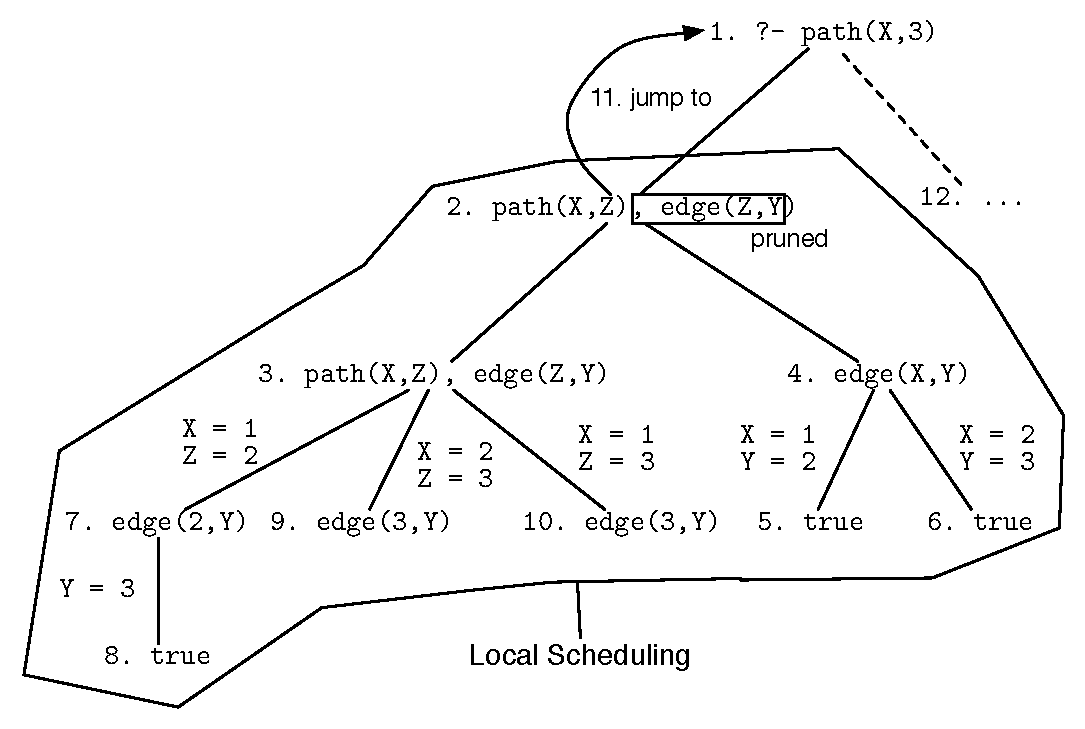
\includegraphics[scale=0.7]{retro_path.pdf}
  \caption{Evaluating `\texttt{path(X,3)}' using retroactive tabling.}
  \label{fig:retro_path}
\end{figure}

\subsection{Multiple Internal Pruning}

An important aspect in internal pruning is \textit{multiple internal pruning}.
Consider that a subgoal $R_1$ calls recursively internal subgoals $R_1, R_2, ..., R_n$ until a subgoal
$S$ is called that subsumes $R_1, R_2, ..., R_n$. In such cases, we ignore all intermediate subgoals
and answers are only pushed from $S$ to $R_1$, the top subgoal. 
For an example, consider the query goal `\texttt{p(1,X)}' and the program in Figure~\ref{fig:retro_multiple_internal_program}.

\begin{figure}[ht]
\begin{Verbatim}
:- use_retroactive_tabling p/2.

p(1,X) :- p(2,X).
p(2,X) :- p(X, _).
p(2,4).
p(1,5).
\end{Verbatim}
\caption{Example program illustrating multiple internal pruning.}
\label{fig:retro_multiple_internal_program}
\end{figure}

Execution starts by storing generator nodes for \texttt{p(1,X)} and \texttt{p(2,X)} and then
\texttt{p(2,X)} calls \texttt{p(X,\_)} that subsumes both \texttt{p(1,X)} and \texttt{p(2,X)}.
Pruning is done between the top subsumed subgoal \texttt{p(1,X)} and the subsuming subgoal
\texttt{p(X,\_)} and the node for \texttt{p(2,X)} is ignored (Figure~\ref{fig:retro_multiple_internal1}).
The choice point for \texttt{p(1,X)} is transformed into a retroactive node and execution proceeds by
applying local scheduling to evaluate \texttt{p(X,\_)}.

\begin{figure}[ht]
  \centering
    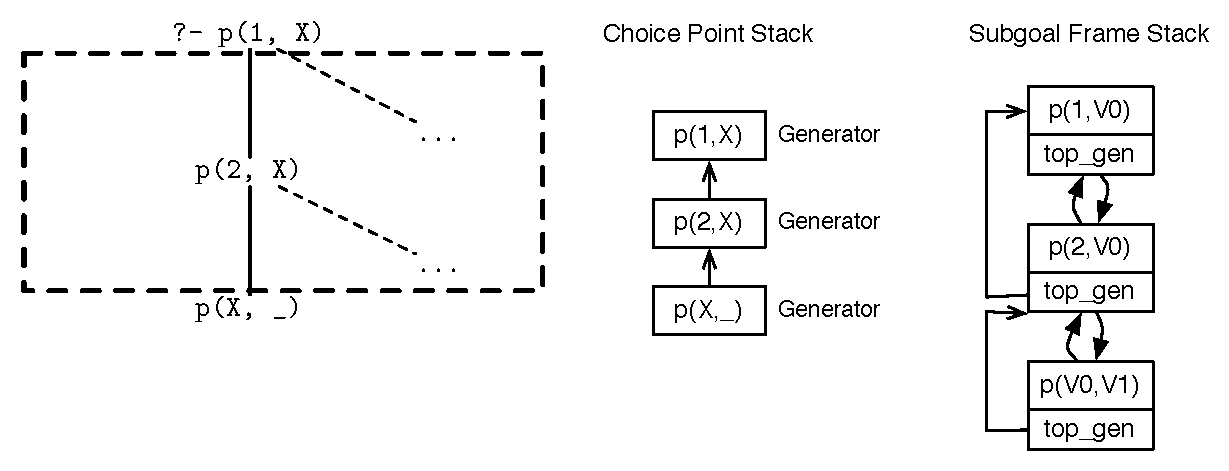
\includegraphics[scale=0.6]{retro_multiple_internal1.pdf}
  \caption{Before multiple internal pruning.}
  \label{fig:retro_multiple_internal1}
\end{figure}

After \texttt{p(X,\_)} fully evaluates with the answers
\texttt{\{X~=~1,~Y~=~4\}},
\texttt{\{X~=~1,~Y~=~1\}},
\texttt{\{X~=~1,~Y~=~2\}},
\texttt{\{X~=~1,~Y~=~5\}},
\texttt{\{X~=~2,~Y~=~1\}},
\texttt{\{X~=~2,~Y~=~2\}},
and finally \texttt{\{X~=~2,~Y~=~4\}}.
Execution is resumed at the retroactive node of
subgoal \texttt{p(1,X)}, where the answers
\texttt{\{X~=~1\}},
\texttt{\{X~=~2\}},
\texttt{\{X~=~4\}},
and \texttt{\{X~=~5\}}
are loaded
(Figure~\ref{fig:retro_multiple_internal2}).
While the subgoal \texttt{p(2,X)} did not participate in later phase of the computation, it has been completed
during the computation of \texttt{p(X,\_)}. 

\begin{figure}[ht]
  \centering
    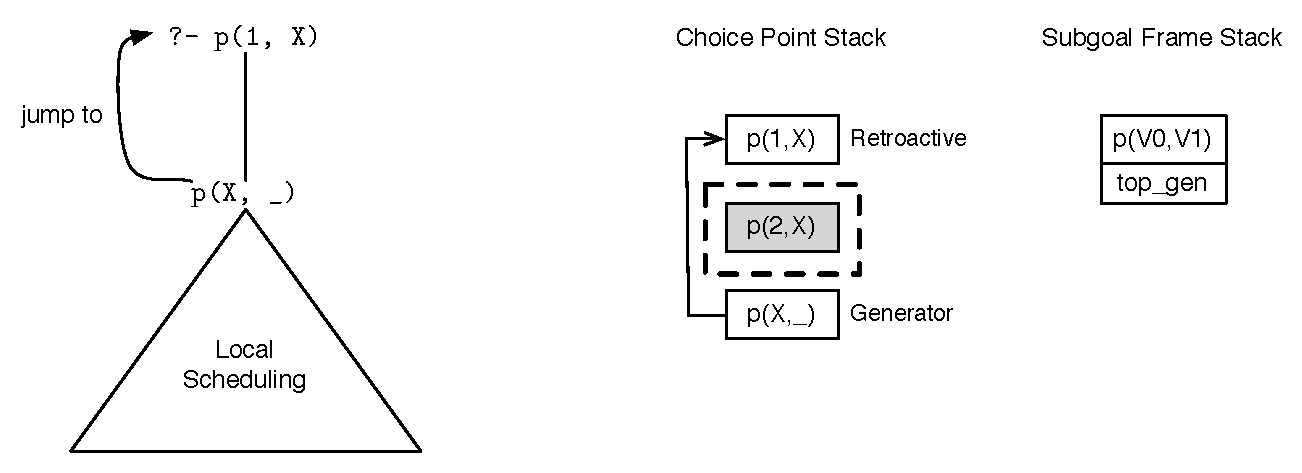
\includegraphics[scale=0.6]{retro_multiple_internal2.pdf}
  \caption{After the evaluation of \texttt{p(X,\_)}.}
  \label{fig:retro_multiple_internal2}
\end{figure}

\section{Mixing External and Internal Pruning}

Although internal and external pruning form the basis of Retroactive Call Subsumption, rules must
be devised in order to prune multiple subgoals that combine both types of pruning. We want to
the minimize the number of pruned subgoals in such a way that a choice point is pruned at
most one time.

Figure~\ref{fig:prune_subgoal_list} shows the \texttt{prune\_subgoal\_list} procedure that accepts
as arguments the subsuming subgoal and the list of subgoals to prune.
First, we compute the oldest internal subgoal $O$ in the set of subgoals and discard other internal
subgoals (phase 1). By using the multiple internal pruning principle (Observation \ref{internal_obs}),
we can prune only the oldest subgoal
because pruning the oldest subgoal will also prune the other internal subgoals as a side-effect.
Notice that we also change the subgoal frame type of all subsumed subgoals to \texttt{RETROACTIVE\_CONSUMER}
and update the \textbf{producer} field to point to the subsuming subgoal.

\begin{samepage}
\begin{pruning_obs}\label{internal_obs}
Let $R_1, R_2, ..., R_n$ be a set of subgoals that are recursively internal. In order to prune the subgoals
$R_1, R_2, ..., R_n$, only the top subgoal, $R_1$, needs to be pruned.
\end{pruning_obs}
\end{samepage}

Next, in phase 2 we check if the list of subgoals is empty, that is, if no external subgoals exist in the list
because internal subgoals have been removed from it in phase 1. Affirmatively, we return early from the procedure
by doing an internal pruning.

In phase 3, we remove all internal subgoal frames that are internal to the subgoal frame $O$ found in phase 1.
Because we will prune the computation of $O$, every subgoal internal to $O$ will be pruned
(except the subsuming subgoal), thus there is no need to prune the two subgoals separately
(Observation~\ref{external_obs}). Next, we finally do an internal pruning using the $O$ subgoal frame
and the resulting list at this point will be empty or contain only external subgoal frames not internal to
$O$ where external pruning must be applied.

\begin{pruning_obs}\label{external_obs}
Let $G$ be a subgoal and $G'$ a subgoal internal to $G$. If $G$ is pruned, $G'$ is also pruned.
\end{pruning_obs}

If the list of subgoals is not empty, we iterate over each external subgoal frame to remove the subgoal frame if
it is internal to another one in the list (phase 4). This is also based on Observation~\ref{external_obs}.
Finally, in phase 5 we apply external pruning to each remaining external subgoal.

For an example, consider the program in Figure~\ref{fig:retro_mix_program} and the query goal
`\texttt{p(2,X),~p(4,Y)}'. Initially, execution creates the generator \texttt{p(2,X)} followed by the internal
generator \texttt{p(3,X)}. Next, the subgoal \texttt{p(4,Y)} is called and the first alternative calls the
subgoal \texttt{p(\_,Y)}, which subsumes every other subgoal (Figure~\ref{fig:retro_mix_multiple_before}).

\begin{figure}[ht]
\begin{Verbatim}
:- use_retroactive_tabling p/2.

p(2, X) :- p(3, X).
p(2, 1).
p(3, 2).
p(3, 5).
p(4, X) :- p(_, X).
p(4, 7).
\end{Verbatim}
\caption{Example program illustrating multiple pruning.}
\label{fig:retro_mix_program}
\end{figure}

By following the rules we previously defined, the oldest internal subgoal we find is \texttt{p(4,X)}.
Next, we filter subgoals that are internal to \texttt{p(4,X)}, but no such subgoals exist. Computation is
then internally pruned by the subgoal \texttt{p(4,X)} and then we must deal with external subgoals.

\begin{figure}[ht]
  \centering
    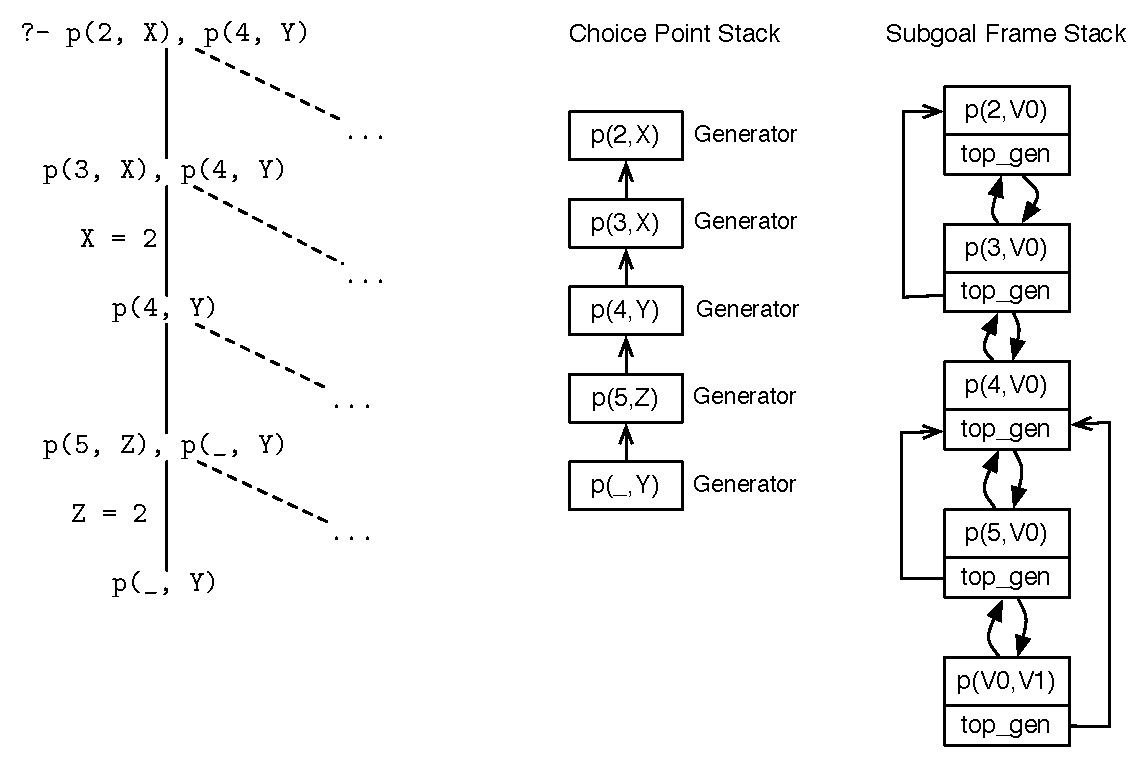
\includegraphics[scale=0.6]{retro_mix_multiple_before.pdf}
  \caption{Before pruning with the subgoal \texttt{p(\_,Y)}.}
  \label{fig:retro_mix_multiple_before}
\end{figure}

The remaining external subgoals are \texttt{p(2,X)} and \texttt{p(3,X)}. Here we must ignore any subgoal
that is internal to any external subgoal. The subgoal \texttt{p(3,X)} matches these conditions and, is thus
removed. Finally, the only remaining subgoal, \texttt{p(2,X)}, is then externally pruned and the computation
can continue as normal.

\begin{figure}[ht]
  \centering
    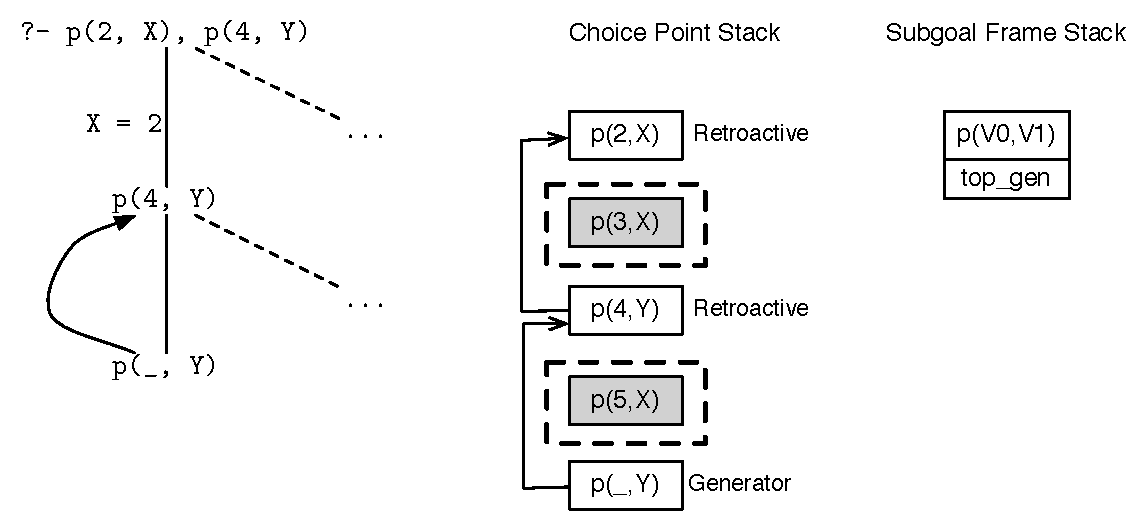
\includegraphics[scale=0.6]{retro_mix_multiple_after.pdf}
  \caption{After pruning with the subgoal \texttt{p(\_,Y)}.}
  \label{fig:retro_mix_multiple_after}
\end{figure}

\begin{figure}[ht]
\begin{Verbatim}
prune_subgoal_list(subsuming, list) {
  if (empty(list))
    return
    
  // phase 1: locate oldest internal subgoal to prune
  min_internal_sg = NULL
  foreach (subgoal in list)
    // change type of subgoal frame and producer
    type(subgoal) = RETROACTIVE_CONSUMER
    producer(subgoal) = subsuming
    
    if (is_internal(subgoal))
      if (min_internal_sg == NULL or
            older_than(generator_cp(subgoal), generator_cp(min_internal_sg)))
        min_internal_sg = subgoal
      
      remove_from_list(list, subgoal)
  
  // only external subgoals in 'list'
  
  // phase 2: return early by checking the existance of external subgoals
  if (empty(list))
    // no external subgoals
    internal_prune(subsuming, min_internal_sg)
    return
  
  if (min_internal_sg)
    // phase 3: filter external subgoals internal to 'min_internal_sg'
    foreach (subgoal in list)
      if (is_internal_subgoal_frame(min_internal_sg))
        remove_from_list(list, subgoal)
    
    // internal prune with 'min_internal_sg'
    internal_prune(subsuming, min_internal_sg)
  
  if (!empty(list))
    // phase 4: remove external subgoals that are
    // internal to other subgoals in 'list'
    foreach (subgoal in list)
      if (is_internal_to_set(subgoal, list))
        remove_from_list(subgoal)
    
    // phase 5: now use the remaining and mutually exclusive
    // external subgoals to apply external pruning
    foreach (subgoal in list)
      external_prune(subsuming, subgoal)
}
\end{Verbatim}
\caption{Pseudo-code for procedure \texttt{prune\_subgoal\_list}.}
\label{fig:prune_subgoal_list}
\end{figure}

\section{Table Space}

Once a pruned subgoal is reactivated and transformed into a loader or consumer node
through retroactive resolution, it is important to avoid consuming answers that
were generated when the subgoal was a generator. When a node consumes less answers,
less code will be executed, thus making execution faster.

In order to efficiently identify what answers have already been used, we designed
the \textit{Single Time Stamped Trie} (STST) table space organization.
In STST we have a common answer trie to all subgoal calls for the predicate. This approach
reduces memory usage and permits easy sharing of answers between subgoals, because an
answer can be referenced by various subgoals.

In this new table space organization, each predicate has two tries, the subgoal trie and
the STST, while each subgoal frame has the answer return list to reference answers
from the STST.
Figure~\ref{fig:stst} illustrates an example of the new table space with the
subgoals \texttt{p(1,VAR0)}, \texttt{p(2,VAR0)} and \texttt{p(VAR0,VAR1)}.

\begin{figure}[ht]
  \centering
    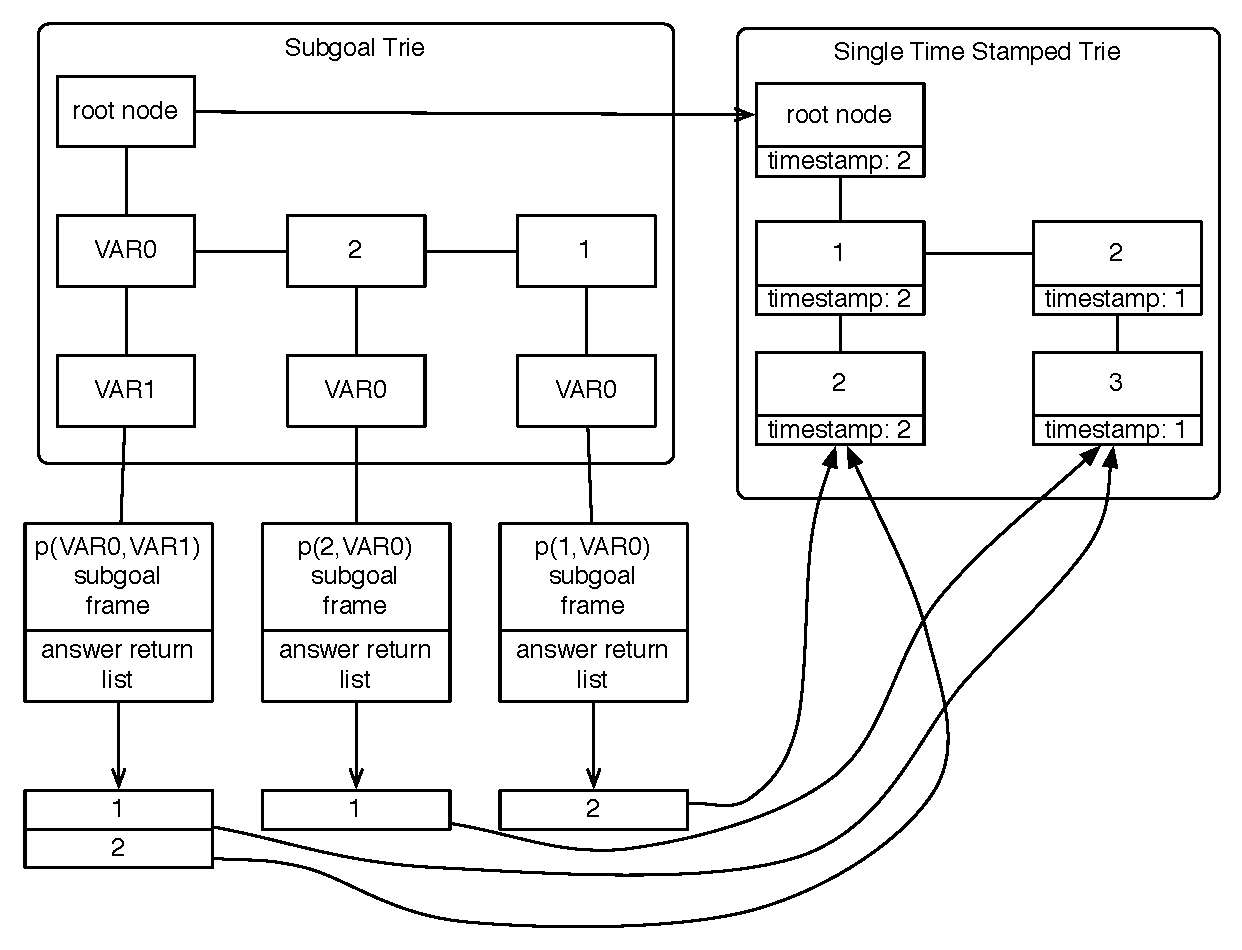
\includegraphics[scale=0.6]{stst.pdf}
  \caption{Example Single Time Stamped Trie.}
  \label{fig:stst}
\end{figure}

In terms of implementation, the STST is stored on the \textbf{next} field of the root
trie node of the subgoal trie. The time stamp of the answer trie can be accessed by
using the root answer trie node.

For subgoal frames, we extended each retroactive subgoal
frame with a \textbf{timestamp} field that stores the time stamp of the last answer
generated or consumed.
The time stamp mechanism helps us identify, using the answer return list, what answers
are relevant to the subgoal from all the answers with the time stamp between 0 and
\textbf{timestamp}. Then, when we need to turn a subgoal frame from generator to consumer,
we can collect answers by using the time stamp stored in the subgoal frame, which was the
time stamp of the last answer successfully inserted on the STST.

\subsection{Answer Templates}

On a traditional call subsumption engine that uses an answer trie per generator subgoal,
the answer template of the consumer subgoal is built dependent of the generator subgoal.
For \textit{retroactive answer templates}, the answer template is simply built by copying
the argument registers of the WAM. This is a very efficient operation compared to traditional
call subsumption methods.

We clearly need the full answer template because the answers on the trie are fully
instantiated on all the predicate arguments, hence the collection and unification of
relevant answers must be seen as unifying against the most general subgoal.

\subsection{Reusing of Answers}

The STST approach also allows reusing answers when a new subgoal is called.
As an example, consider that two unrelated (no subsumption involved) subgoals $S_1$
and $S_2$ are fully evaluated. If a subgoal $S$ is then called, it is possible
that some of the answers on the STST match $S$ even if $S$ neither subsumes
$S_1$ or $S_2$. Hence, instead of eagerly running the predicate clauses, we start
by loading the matching answers already on the STST, which can be enough if,
for example, $S$ gets pruned by a cut. This is a similar approach to the \textit{incomplete
tabling} approach for tabling with variant checks \cite{Rocha-06a}.

While the reusing of answers has some advantages, it can lead to redundant computations.
This happens when $S$ generates more general answers than the ones initially
loaded when using traditional call subsumption. For an example, consider the retroactive
tabled predicate \texttt{p/1} with only one fact, '\texttt{p(X)}`. If \texttt{p(1)} is
called, the answer represented as \texttt{\{ARG0~=~1\}} is added on the STST and execution
would return \texttt{true}. If the subgoal \texttt{p(X)} was now called, we would search
the STST for relevant answers and the first answer would be \texttt{\{X~=~1\}}. If we
asked for more answers, the system would return a new answer, \texttt{true}, and add it
to the STST (Figure~\ref{fig:stst_redundant}). If we called
\texttt{p(X)} with an empty STST, only one answer would be returned, \texttt{true}.

\begin{figure}[ht]
  \centering
    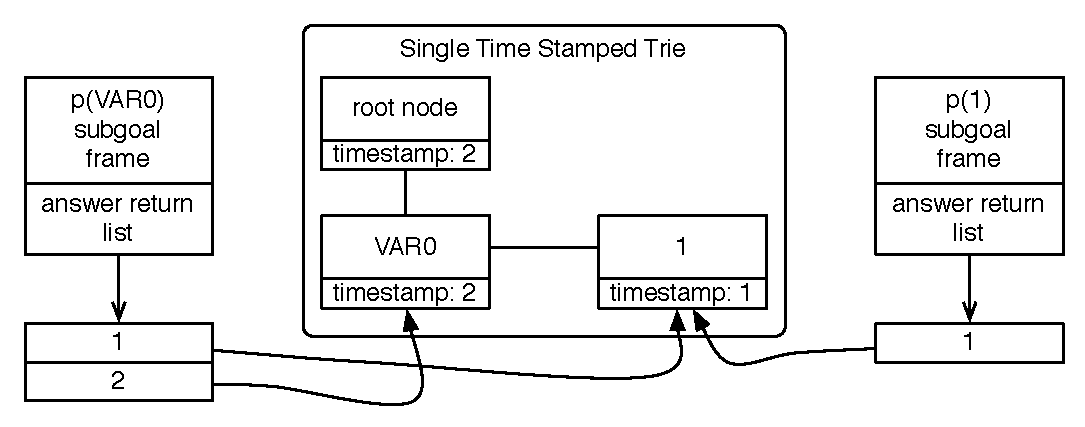
\includegraphics[scale=0.6]{stst_redundant.pdf}
  \caption{Answer redundancy with STST.}
  \label{fig:stst_redundant}
\end{figure}

\subsection{Insertion of Answers}

The insertion of answers on a STST works the same as standard TSTs, but special care
must be taken when inserting an answer and updating the subgoal frame \textbf{timestamp}
field.
When only one subgoal is adding answers on the STST, the subgoal frame time stamp
gets incremented each time an answer is inserted. Repeated answers are easily recognized
by testing if the answer is new or not.
The problem arises when various subgoals are inserting answers, thus it may be difficult
to determine if an answer is repeated for a certain subgoal.

Let's consider that two subgoals $S1$ and $S2$ are currently
evaluating and each one can insert a new answer on the STST at any time (see
Figure~\ref{fig:stst_conflicts}). $S1$ generates the first 3 answers (time stamp 3)
and evaluation initiates in subgoal $S2$. Here, we do not find any answers relevant
for $S2$ on the STST and the evaluation of program clauses results in three new answers,
4, 5 and 6. The time stamp of $S2$ is thus updated to 6.

Next, if $S1$ now generates the answer 5 we can incorrectly detect a repeated answer
for this subgoal if we consider that repeated answers on the STST are repeated answers for the
subgoal (which are not). We could also consider it a new answer, since the old $S1$ time stamp
is in the past ($3 < 5$). But this will still arise problems after we update $S1$ time stamp
to either 6 (the global time stamp) or 5 (the newer answer time stamp for the subgoal).
If answer 4 is also relevant for $S1$, it will be considered a repeated answer
during its insertion. Therefore, we need a more complex mechanism to
detect repeated answers per subgoal.

\begin{figure}[ht]
  \centering
    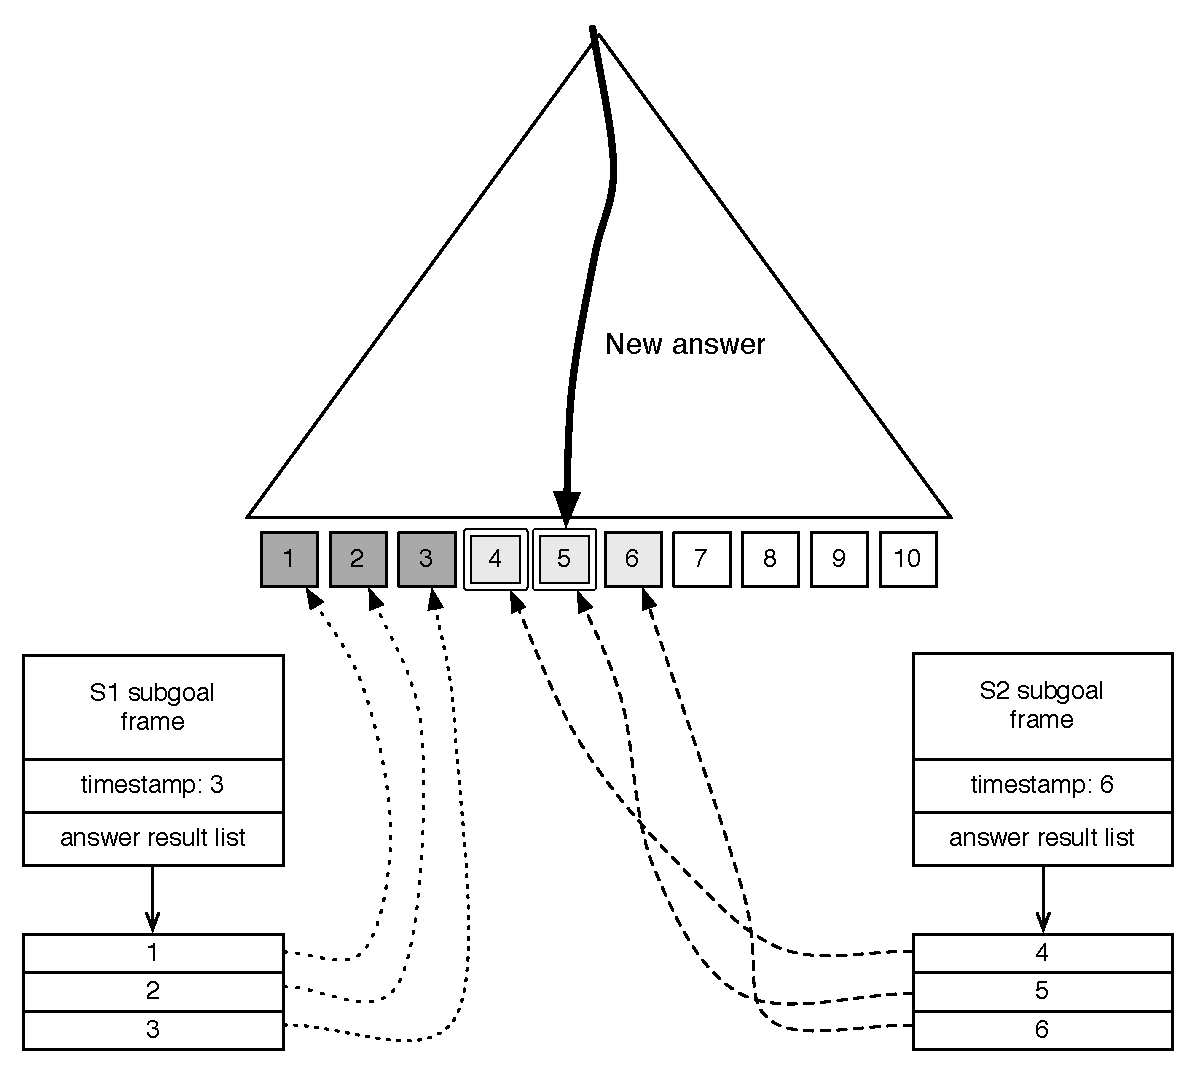
\includegraphics[scale=0.5]{stst_conflicts.pdf}
  \caption{Insertion conflicts of answers on a STST.}
  \label{fig:stst_conflicts}
\end{figure}

In our new approach, we create a \textit{pending answer index} for each subgoal frame.
This index contains all the answers that are older than the subgoal frame time stamp
and were still not generated by the subgoal. This indexed is created whenever the STST
global time stamp is greater than the current subgoal frame time stamp. It is built by
collecting all the relevant answers for the subgoal frame starting from the current
subgoal frame time stamp. Then, whenever an answer appears on the past, we look up on the
pending answer index to check if the answer is there. If the answer is really there,
we consider it a new answer; if not, we consider it a repeated answer. In both cases
the answer is removed from the index.

The pending answer index is implemented as a single linked list, but can be transformed
into an hash table if the linked list gets too big. Also, the hash table is dynamically
resized after a certain threshold, in order to maintain good access times.

Figure~\ref{fig:stst_insert} presents the code for the \texttt{stst\_insert} procedure,
which inserts the answer on the STST and sets the \textbf{status} field bit indicating
if the answer must be inserted into the answer return list of the subgoal frame. The
pseudo-code is organized into four cases:

\begin{enumerate}
   \item Answers are inserted in order and only one subgoal is adding answers.
   This happens in the majority of the situations.
   \item One answer was inserted by another subgoal and it is the only answer that
   the current subgoal has still not considered. It is trivially set as a new answer.
   \item The answer time stamp is older than the subgoal frame time stamp, therefore
   the pending answer index must be inspected.
   \item The answer time stamp is younger than the subgoal frame time stamp $t$, thus
   we must collect the relevant answers beginning from $t$ and add them into the pending
   answer index, except the current answer.
\end{enumerate}

\begin{figure}[ht]
\begin{Verbatim}
stst_insert(subgoal_fr, answer) {
  table_entry = table_entry(subgoal_fr)
  stst = answer_trie(table_entry)
  old_timestamp = timestamp(stst)
  leaf_node = subsumptive_answer_search(stst, answer)
  new_timestamp = timestamp(stst)
  
  if (old_timestamp == new_timestamp - 1 and
        timestamp(subgoal_fr) == old_timestamp)
    // case 1: new, incremental, answer
    set_new_answer(leaf_node)
    timestamp(subgoal_fr) = new_timestamp
  else if (old_timestamp == new_timestamp and
        timestamp(subgoal_fr) == old_timestamp - 1 and
        timestamp(leaf_node) == new_timestamp)
    // case 2: one new answer inserted by someone else
    // and no answers were left behind
    set_new_answer(leaf_node)
    timestamp(subgoal_fr) == new_timestamp
  else if (timestamp(leaf_node) <= timestamp(subgoal_frame))
    // case 3: answer is in the past,
    // check if it must be considered new
    if (locate_pending_answer(subgoal_sf, leaf_node))
      set_new_answer(leaf_node)
    else
      set_old_answer(leaf_node)
  else
    // case 4: answers were inserted by someone else
    pending_list = tst_collect_relevant_answers(stst, timestamp(subgoal_fr),
            answer_template(subgoal_fr))
    
    remove_from_list(answer_list, leaf_node)
    add_pending_answers(subgoal_sf, pending_list)
    set_new_answer(leaf_node)
    timestamp(subgoal_fr) = new_timestamp
}
\end{Verbatim}
\caption{Pseudo-code for procedure \texttt{stst\_insert}.}
\label{fig:stst_insert}
\end{figure}

It is important to note that when a generator subgoal frame is transformed into a
consumer subgoal frame, we must remove all the answers from the pending answer index
and insert them on the answer return list. Therefore, all the consumer mechanisms
can still work normally, without awareness of the pending answer index.

\subsection{Compiled Tries and Completed Table}

Our system only compiles the STST when the most general subgoal is completed.
This avoids problems when a subgoal is executing compiled code and another
is inserting answers, leading to the loss of answers as hash tables can be
dynamically created and expanded.

We also implemented the \textit{completed table optimization}. This optimization throws
away the subgoal trie and the subgoal frames when the most general subgoal is completed.
When a subgoal call is made, we just build the answer template by copying the argument
registers and then we execute the compiled trie, thus bypassing all the mechanisms of
locating the subgoal on the subgoal trie, leading to memory and speedup gains. 

\section{Searching Subsumed Subgoals}

In order to efficiently find which subsumed subgoals are evaluating and are subsumed
by the called subgoal, we extended the subgoal trie data structure and designed a new
algorithm to search these subgoals.

\subsection{Subgoal Trie Data Structure}

Each subgoal trie node was extended with a new field, named
\textbf{in\_eval}, which stores the number of subgoals, represented below the
node, that are in evaluation. This field is used to, during the search
for subsumed subgoals, prune the subgoal trie branches without
evaluating subgoals, i.e., the ones with $\textbf{in\_eval} = 0$.

When a subgoal starts being evaluated, all subgoal trie nodes in its
subgoal trie path get the \textbf{in\_eval} field incremented. When a subgoal
completes its evaluation, the path is decremented. Hence, for each
subgoal leaf trie node, the \textbf{in\_eval} field can be equal to either:
1, when the corresponding subgoal is in evaluation; or 0, when the
subgoal is completed. For the root subgoal trie node, we know that it
will always contain the total number of subgoals being currently
evaluated. For an example, consider the subgoal trie in
Fig.~\ref{fig:in_eval_trie} representing four evaluating subgoals and
one completed subgoal for a tabled predicate \texttt{p/2}.

\begin{figure}[ht]
\centering
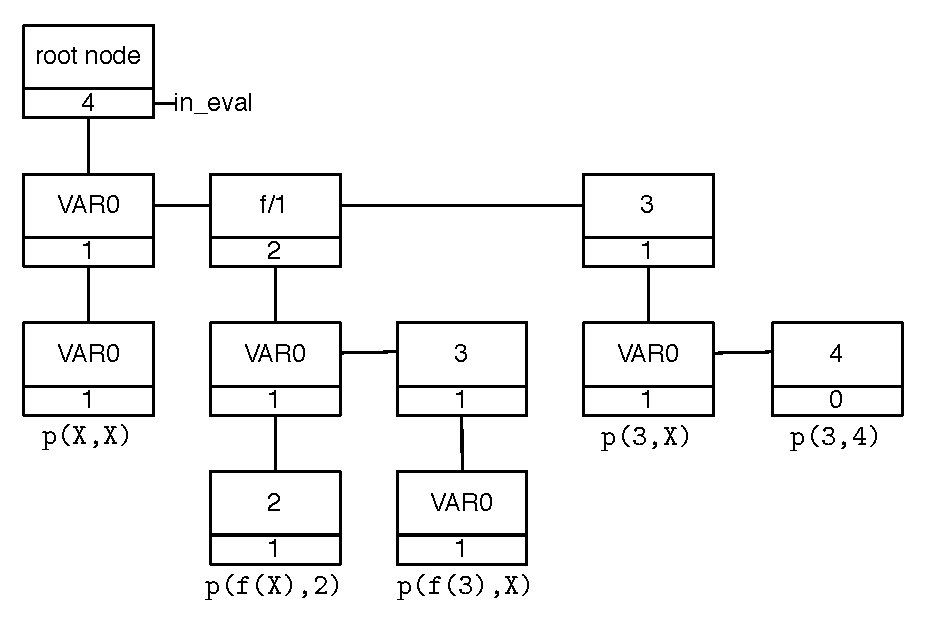
\includegraphics[scale=0.6]{in_eval_trie}
\caption{The \textbf{in\_eval} field in a subgoal trie representing a \texttt{p/2}
  tabled predicate}
\label{fig:in_eval_trie}
\end{figure}

Consider now, that a new subgoal \texttt{p(f(3),5)} enters the
evaluation. One new subgoal trie node is created on the subgoal trie
to represent the new subgoal call and all the trie nodes from the leaf
node to the root node get the \textbf{in\_eval} field incremented
(Fig.~\ref{fig:in_eval_add}). Note also how the root node is
incremented from 4 to 5, meaning that 5 subgoals are now in
evaluation.

\begin{figure}[ht]
\centering
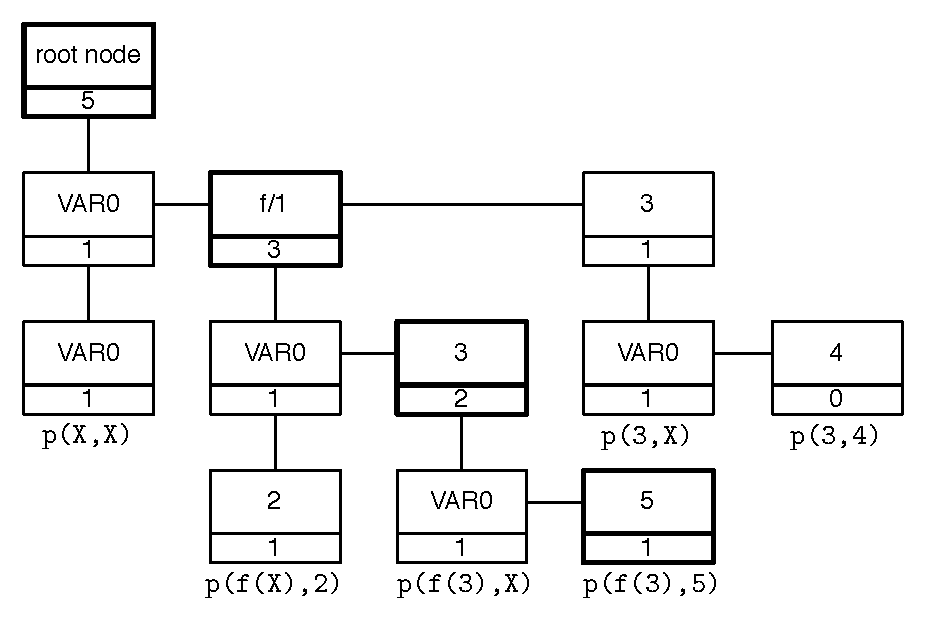
\includegraphics[scale=0.42]{in_eval_add}
\caption{Inserting subgoal \texttt{p(f(3),5)} in the subgoal trie of
  Fig.~\ref{fig:in_eval_trie}}
\label{fig:in_eval_add}
\end{figure}

When a chain of sibling nodes is organized in a linked list, it is
easy to select the trie branches with evaluating subgoals by looking
for the nodes with $\textbf{in\_eval} > 0$. But, when the sibling nodes are
organized in an hash table, it can become very slow to inspect each
node as the number of siblings increase. In order to solve this
problem, we designed a new data structure, called \textit{evaluation
index}, in a similar manner to the time stamp index of the TST design.

An evaluation index is a double linked list that is built for each
hash table and is used to chain the subgoal trie nodes where the
\textbf{in\_eval} field is greater than 0. Note that this linked list is not
ordered by the \textbf{in\_eval} value. Each evaluation index node contains
the following fields: \textbf{prev}, a pointer to the previous evaluation
index node, if any; \textbf{next}, a pointer to the next evaluation index
node, if any; \textbf{node}, a pointer to the subgoal trie node the index
node represents; and \textbf{in\_eval}, the number of evaluating subgoals
under the corresponding subgoal trie node. We also extended the hash
table with a field named \textbf{index} to point to the evaluation index.

Figure~\ref{fig:hash_table_evaluation_index} shows an hash table and
the corresponding evaluation index. Note that an indexed subgoal trie
node now uses the \textbf{in\_eval} field to point to the index node, while a
trie node with $\textbf{in\_eval} = 0$ is not indexed. To compute the
\textbf{in\_eval} value of a trie node, we first use the \textbf{status} field to
determine if the node is inside an hash table or not, and then use the
\textbf{in\_eval} field accordingly.

\begin{figure}[ht]
  \centering
  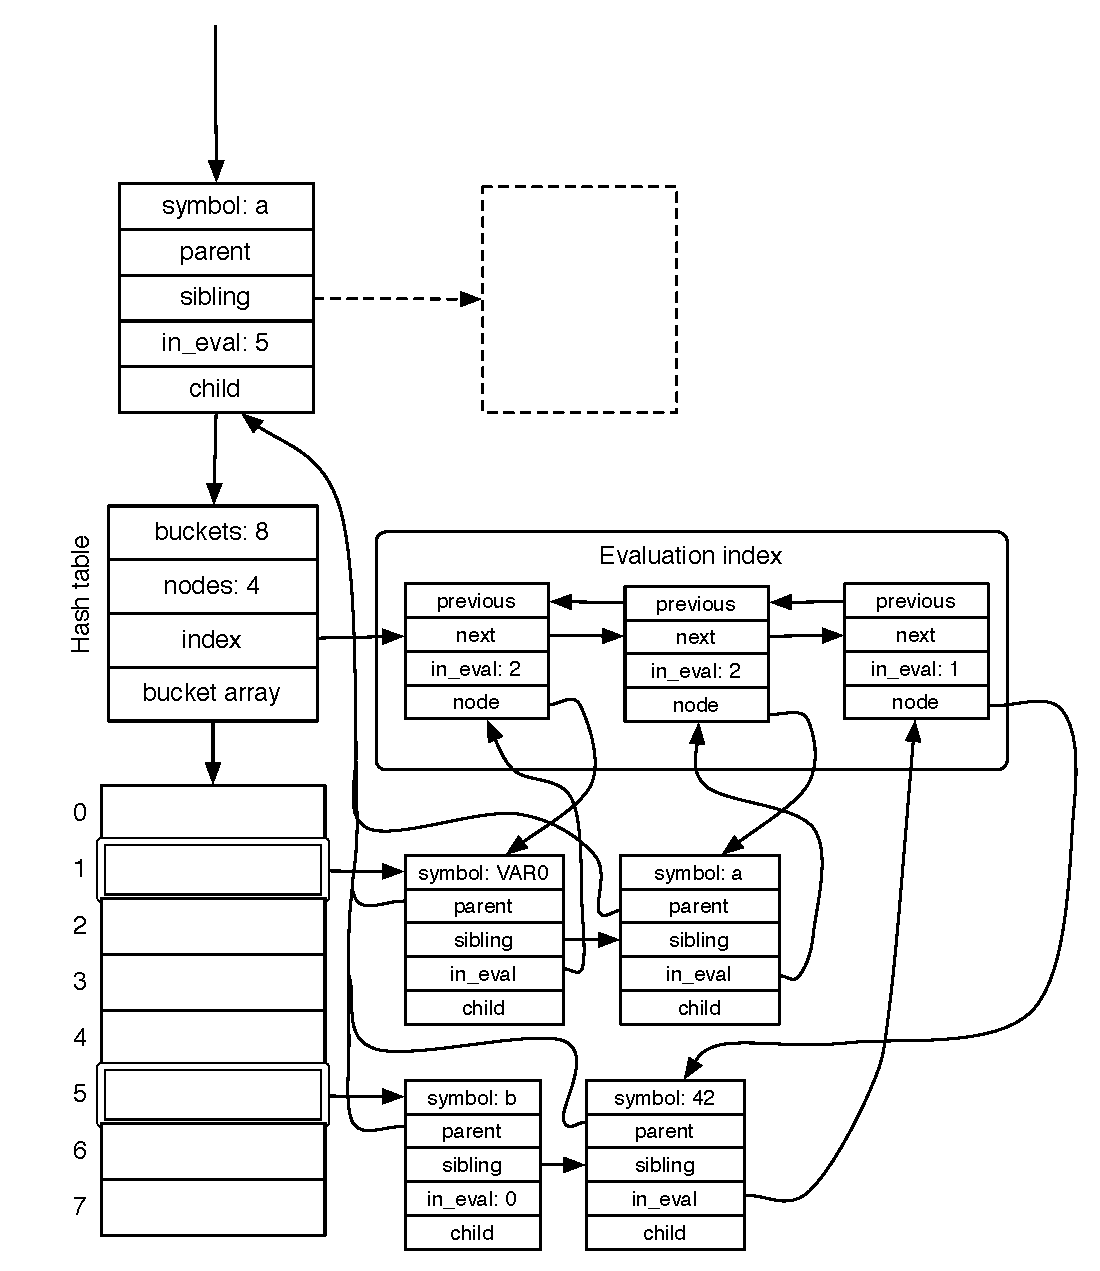
\includegraphics[scale=0.6]{hash_table_evaluation_index.pdf}
  \caption{An hash table with an evaluation index.}
  \label{fig:hash_table_evaluation_index}
\end{figure}

The evaluation index makes the operation of pruning trie branches much
more efficient by providing direct access to trie nodes with
evaluating subgoals. While advantageous, the operation of incrementing
or decrementing a subgoal trie path is more costly, because these
indexes must be maintained.

Figure~\ref{fig:increment_in_eval} presents the pseudo-code for the
\texttt{increment\_in\_eval} procedure. This procedure iterates over the
subgoal trie path and increments the \textbf{in\_eval} field from the leaf to
the root node. When we find hashed trie nodes, we must check if the
node is currently being indexed. If this is the case, we simply
increment the \textbf{in\_eval} field of the index node, otherwise we create
a new index node on the evaluation index pointing to the current
subgoal trie node and the \textbf{in\_eval} field of the subgoal trie node is
made to point to the index node.

\begin{figure}[ht]
\begin{Verbatim}
increment_in_eval(leaf_node, root_node) {
  current_node = leaf_node
  while (current_node != root_node)
    if (is_hashed_node(current_node))
      if (in_eval(current_node) == 0)
        // not indexed
        hash_table = child(parent(current_node))
        index_node = add_index_node(hash_table, current_node)
        in_eval(current_node) = index_node
      else
        // indexed
        index_node = in_eval(current_node)
        in_eval(index_node) = in_eval(index_node) + 1
    else
      // simple chain list
      in_eval(current_node) = in_eval(current_node) + 1
    current_node = parent(current_node)
  in_eval(root_node) = in_eval(root_node) + 1
}
\end{Verbatim}
\caption{Pseudo-code for procedure \texttt{increment\_in\_eval}.}
\label{fig:increment_in_eval}
\end{figure}

Figure~\ref{fig:hash_table_evaluation_index_increment} shows the
resulting hash table and evaluation index if the subgoal trie node in
Figure~\ref{fig:hash_table_evaluation_index} that is not indexed gets
indexed.

\begin{figure}[ht]
  \centering
  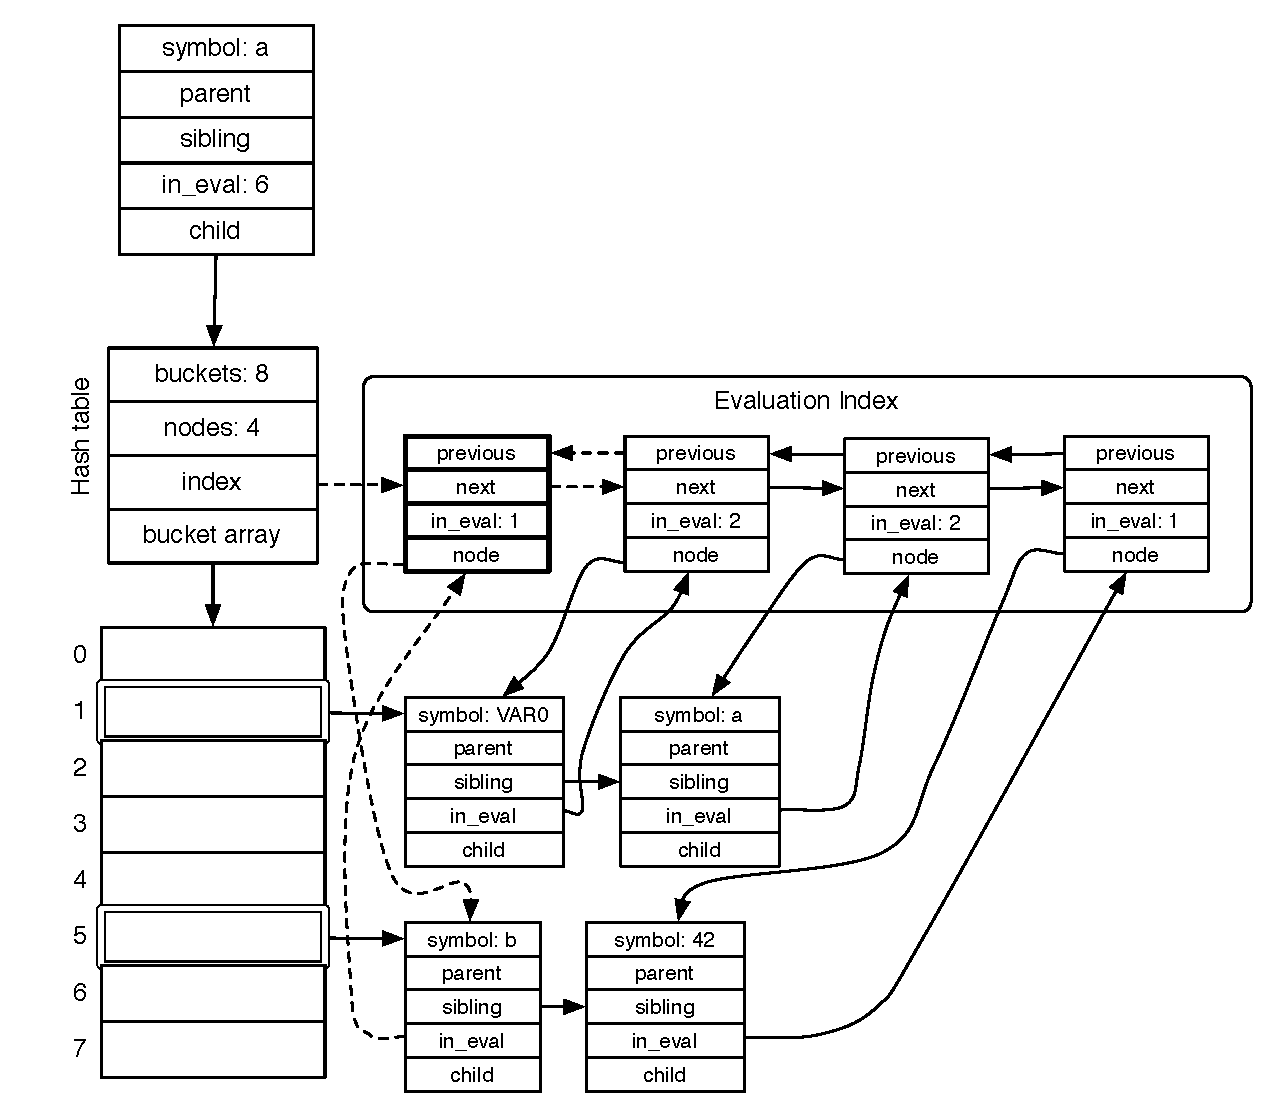
\includegraphics[scale=0.6]{hash_table_evaluation_index_increment.pdf}
  \caption{Indexing a non-indexed subgoal trie node through an evaluation index.}
  \label{fig:hash_table_evaluation_index_increment}
\end{figure}

The procedure in Figure~\ref{fig:decrement_in_eval},
\texttt{decrement\_in\_eval}, does the inverse job of procedure
\texttt{increment\_in\_eval}. When decrementing an indexed subgoal trie
node, if the \textbf{in\_eval} field reaches 0, the trie node no longer needs
to be indexed, and hence we must remove the index node from the
evaluation index. In the other cases, we simply decrement the
respective \textbf{in\_eval} field.

\begin{figure}[ht]
\begin{Verbatim}
decrement_in_eval(leaf_node, root_node) {
  current_node = leaf_node
  while (current_node != root_node)
    if (is_hashed_node(current_node))
      index_node = in_eval(current_node)
      if (in_eval(index_node) == 1)
        // remove from index
        hash_table = child(parent(current_node))
        remove_index_node(hash_table, index_node)
        in_eval(current_node) = 0
      else
        // keep indexed
        in_eval(index_node) = in_eval(index_node) - 1
    else
      // simple chain list
      in_eval(current_node) = in_eval(current_node) - 1
    current_node = parent(current_node)
  in_eval(root_node) = in_eval(root_node) - 1
}
\end{Verbatim}
\caption{Pseudo-code for procedure \texttt{decrement\_in\_eval}.}
\label{fig:decrement_in_eval}
\end{figure}

\subsection{Matching Algorithm}

The algorithm that finds the currently running subgoals that are
subsumed by a more general subgoal $S$ works by matching the subgoal
arguments $SA$ of $S$ against the trie symbols in the subgoal trie
$T$. By using the \textbf{in\_eval} field as described previously, we can
prune irrelevant branches as we descend the trie. When reaching a leaf
node, we append the corresponding subgoal frame in a result list that
is returned once the process finishes. If the matching process fails
at some point or if a leaf node was reached, the algorithm backtracks
to try alternative branches, in order to fully explore the subgoal
trie $T$.

When traversing $T$, trie variables cannot be matched against ground
terms of $SA$. Ground terms of $SA$ can only be matched with ground
terms of $T$. For example, if matching the trie subgoal
\texttt{p(VAR0,VAR1)} with the subgoal \texttt{p(2,X)}, we cannot match the
constant \texttt{2} against the trie variable \texttt{VAR0}, because \texttt{p(2,X)} does
not subsume \texttt{p(X,Y)}.

When a variable of $SA$ is matched against a ground term of $T$,
subsequent occurrences of the same variable must also match the same
term. As an example, consider the trie subgoal \texttt{p(2,4)} and the
subgoal \texttt{p(X,X)}. The variable \texttt{X} is first matched against
\texttt{2}, but the second matching, against \texttt{4}, must fail because
\texttt{X} is already bound to \texttt{2}.

Now consider the trie subgoal \texttt{p(VAR0,VAR1)} and the subgoal
\texttt{p(X,X)}. Variable \texttt{X} is first matched against \texttt{VAR0}, but then we
have a second match against a different trie variable, \texttt{VAR1}. Again,
the process must fail because \texttt{p(X,X)} does not subsume \texttt{p(X,Y)}. This
last example evokes a new rule for variable matching. When a variable
of $SA$ is matched against a trie variable, subsequent occurrences of
the same variable must always match the same trie variable. This is
necessary, because the found subgoals must be \emph{instances} of
$S$. Therefore, this problem can be reduced to the task of finding all
instances of $S$ in trie $T$. To implement this algorithm, we use the
following data structures:

\begin{itemize}
\item \textit{WAM data structures}: heap, trail, and associated
  registers. The heap is used to build structured terms, in which the
  subgoal arguments or trie variables are bound. Whenever a term
  variable is bound, we trail it using the WAM trail;
\item \textit{term stack}: stores the remaining terms to be matched
  against the subgoal trie symbols;
\item \textit{term log stack}: stores already matched terms from the
  term stack and is used to restore the state of the term stack when
  backtracking;
\item \textit{variable enumerator vector}: used to mark the term
  variables that were matched against trie variables;
\item \textit{choice point stack}: stores choice point frames, where
  each frame contains information needed to restore the computation in
  order to search for alternative branches.
\end{itemize}

Figure~\ref{fig:collect_subsumed_subgoals} shows the pseudo-code for
the procedure that traverses a subgoal trie and collects the set of
subsumed subgoals of a given subgoal call. This procedure can be
summarized in the following steps:

\begin{enumerate}
\item setup WAM machinery and push subgoal arguments into the term
  stack.
\item fetch a term $T$ from the term stack;
\item search for a trie node $N$ where the \textbf{in\_eval} field is not 0.
\item search for the next node with a valid \textbf{in\_eval} field to be
  pushed on the choice point stack, if any;
\item match $T$ against the trie symbol of $N$;
\item proceed into the child of $N$ or, if steps 3 or 5 fail,
  backtrack by popping a frame from the choice point stack and use the
  alternative trie node;
\item once a leaf is reached, add the corresponding subgoal frame to
  the resulting subgoal frame list. If there are choice points
  available, backtrack to try them;
\item if no more choice point frames exist, return the found subsumed
  subgoals.
\end{enumerate}

\begin{figure}[ht]
\begin{Verbatim}
collect_subsumed_subgoals(subgoal_trie, subgoal_call) {
  save_wam_registers()
  push_arguments(term_stack, subgoal_call)
  subgoals = NULL
  parent = subgoal_trie
  node = child(parent)
  while (true)
    term = deref(pop(term_stack))    
    if (is_atom(term) or is_integer(term))
      try_node = try_constant_term(term, node)
    else if (is_functor(term) or is_list(term))
      try_node = try_structured_term(term, node)
    else if (is_variable(term))
      try_node = try_variable_term(term, node)
    if (try_node != NULL)
      push(term_log_stack, term)
      parent = try_node
      node = child(parent)
      if (empty(term_stack))                // new subsumed subgoal found
        add_subgoal(subgoals, subgoal_frame(parent))
      else
        continue
    if (empty(choice_point_stack))
      unwind_wam_trail()
      restore_wam_registers()
      return subgoals
    else
      node = pop_choice_point_frame(choice_point_stack)
      parent = parent(node)
}
\end{Verbatim}
\caption{Pseudo-code for procedure \texttt{collect\_subsumed\_subgoals}.}
\label{fig:collect_subsumed_subgoals}
\end{figure}

\subsection{Choice Point Stack}

To store alternative branches for exploration, we use a choice point stack.
Each choice point frame
(see Figure~\ref{fig:choice_point_stack2})
stores the following fields:
\textbf{alt\_node}, the alternative node to explore;
\textbf{term\_stack\_top}, the top of the term stack;
\textbf{term\_log\_stack\_top}, the top of the term log stack;
\textbf{trail\_top}, the current trail position;
and \textbf{saved\_HB}, the register HB. Note that we used the same choice point stack
from Section~\ref{sec:cpstack_section}.

\begin{figure}[ht]
  \centering
    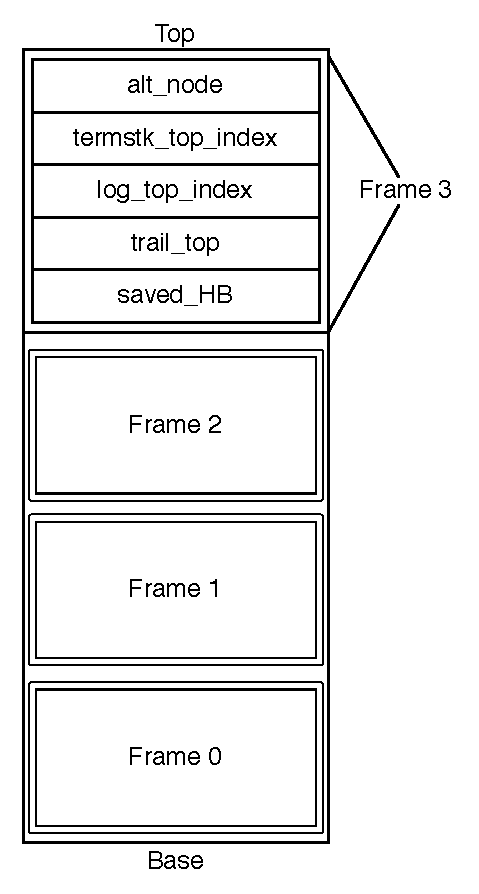
\includegraphics[scale=0.5]{choice_point_stack.pdf}
  \caption{Choice point stack organization.}
  \label{fig:choice_point_stack2}
\end{figure}

The HB register is used to detect conditional bindings in same manner as for the HB register in
WAM choice points, that is, we use it do know if a term variable needs to be trailed.
When a choice point frame is popped from the stack, the state of the computation is restored
by executing the following actions:

\begin{itemize}
\item the current node and parent node are reset;
\item all terms stored in the term log stack are pushed back to the
  term stack;
\item the trail is unwound to reset the variables that were bound
  after choice point creation;
\item registers H and HB are reset to their previous values.
\end{itemize}

Since constant and structured terms can have at most one matching
alternative in a trie level, choice point frames are only pushed when
the current term is a variable. Remember that if a node satisfies the
\textbf{in\_eval} requisite, variable terms can match all types of trie
symbols, including trie variables.

\subsection{Matching Constant and Structured Terms}

If the next term from the term stack is a constant or a structured
term we must match it against a similar ground term only. Both
constant and structured terms work pretty much the same way, except
that for a list or a functor term we push the term arguments into the
term stack before descending into the next trie level. The arguments
are pushed into the stack in order to be matched against the next trie
symbols.

Figure~\ref{fig:try_structured_term} presents the pseudo-code for the
\texttt{try\_structured\_term} procedure. This procedure is divided into
two steps. We arrive at step 1, if the current node is an hash
table. Here, first, we hash the term to get the hash bucket that might
contain the matching trie node. If the bucket is empty we simply
return \texttt{NULL}. Otherwise, we move into step 2. In step 2 we traverse a
chain of sibling nodes (a simple chain or a bucket chain) looking for
a node with a matching symbol and with a valid \texttt{in\_eval} value.

\begin{figure}[ht]
\begin{Verbatim}
try_structured_term(term, current_node)
  if (is_hash_table(current_node))
    // step 1: check hash bucket
    hash_table = current_node
    current_node = bucket_array(hash_table, term)
    if (current_node == NULL)
      return NULL
  foreach (node in current_node)
    // step 2: traverse chain of sibling nodes
    if (symbol(node) == term)
      if (in_eval(node) > 0)
        push_arguments(term_stack, term)
        return node
      else
        // no running subgoals below
        return NULL
  return NULL
}
\end{Verbatim}
\caption{Pseudo-code for procedure \texttt{try\_structured\_term}.}
\label{fig:try_structured_term}
\end{figure}

\subsection{Matching Variable Terms}

A variable term can potentially be matched against any trie symbol. It
is only when the variable is matched against a trie variable that the
process may fail. Figure~\ref{fig:try_variable_term} shows the
pseudo-code for the \texttt{try\_variable\_term} procedure. It is defined
by three main cases, depending on the type of the current node,namely:

\begin{enumerate}
\item the node is an hash table. For faster access of valid trie  nodes, we use the evaluation index, which gives us all the valid
  trie nodes in a linked list. We set the next alternative node to be  pushed on the choice point stack by using the function
  \texttt{next\_valid\_index\_node} that uses the \textbf{next} pointer of the  first index node to locate the alternative trie node.
\item the node is an hashed node, thus is on the evaluation index of  the corresponding hash table. In this case, we also use the
  \texttt{next\_valid\_index\_node} function to identify the next
  alternative trie node.\item the node is part of a simple linked list. Here we must use the
  function \texttt{next\_valid\_node} to find the next valid trie node
  ($\textbf{in\_eval} > 0$). The alternative trie node is also set using this
  function on the sibling node.
\end{enumerate}

\begin{figure}[ht]
\begin{Verbatim}
try_variable_term(variable, current_node) {
  if (is_hash_table(current_node))
    // case 1: hash table
    hash_table = current_node
    index_node = index(hash_table)    
    if (index_node == NULL)
      // no running subgoals below
      return NULL    
    current_node = node(index_node)
    alt_node = next_valid_index_node(current_node)
  else if (is_hashed_node(current_node))
    // case 2: indexed node
    alt_node = next_valid_index_node(current_node)
  else
    // case 3: simple chain list
    current_node = next_valid_node(current_node)
    if (current_node == NULL)
      return NULL
    alt_node = next_valid_node(current_node)
  push_choice_point_frame(choice_point_stack, alt_node)
  if (try_variable_matching(variable, symbol(current_node)))
    return current_node
  else
    return NULL
}
\end{Verbatim}
\caption{Pseudo-code for procedure \texttt{try\_variable\_term}.}
\label{fig:try_variable_term}
\end{figure}

After the current valid node and alternative node are set, we push the
alternative into the choice point stack and call the
\texttt{try\_variable\_matching} procedure (Figure~\ref{fig:try_variable_matching})
to match the term variable with the trie node symbol.

\begin{figure}[!ht]
\begin{Verbatim}
try_variable_matching(symbol, variable, node) {
 if (is_variable(symbol))
   if (is_in_variable_enumerator_vector(variable))
     enumerator_index = enumerator_index(variable)
     var_index = var_index(symbol)
     return enumerator_index == var_index
   else
     // new term variable
     var_index = var_index(symbol)
     mark_variable_enumerator_vector(variable, var_index)
     return TRUE
 else
   // non-variable symbol
   if (is_in_variable_enumerator_vector(variable))
     // variable must be matched against the same trie variable
     return FALSE
   if (is_constant(symbol))
     bind_and_conditionally_trail(variable, symbol)
   else if (is_functor(symbol) or is_list(symbol))
     term = create_heap_structure(symbol)
     bind_and_conditionally_trail(variable, term)
     push_arguments(term_stack, deref(variable))
   else
     return FALSE
}
\end{Verbatim}
\caption{Pseudo-code for procedure \texttt{try\_variable\_matching}.}
\label{fig:try_variable_matching}
\end{figure}

Matching a term variable with a trie symbol depends on the type of the
trie symbol. If the trie symbol is a trie variable, we have two cases.
If the term variable is free (i.e., this is its first occurrence), we
simply make it to point to the position on the variable enumerator
vector that corresponds to the trie variable index and we trail the
term variable using the WAM trail. Otherwise, the term variable is
already matched against a trie variable (on the variable enumerator
vector), thus we get both indexes (term and trie variable indexes) and
the matching succeeds if they correspond to the same index (same
variable).

If the trie symbol is a ground term, we must verify if the term
variable is on the variable enumerator vector and, in such case, we
must fail. Term variables matched against trie variables must only be
matched against the same trie variable. Otherwise, for constant trie
symbols, we simply bind the term variable to the trie symbol. For
structured terms (lists and functors), we create the structured term
on the heap, bind the term variable to the heap address, and push the
new term arguments into the term stack to be matched against the next
trie symbols.

\subsection{Example Execution}

Consider the subgoal trie with three executing subgoals represented in
Figure~\ref{fig:example_trie}. We want to retrieve subgoals that are
subsumed by the subgoal \texttt{p(X,2,X)}. Initially, the algorithm setups
the WAM registers and then pushes the subgoal arguments into the term stack
resulting in the following stack configuration (from bottom to top): \texttt{[X,2,X]}.

\begin{figure}[ht]
\centering
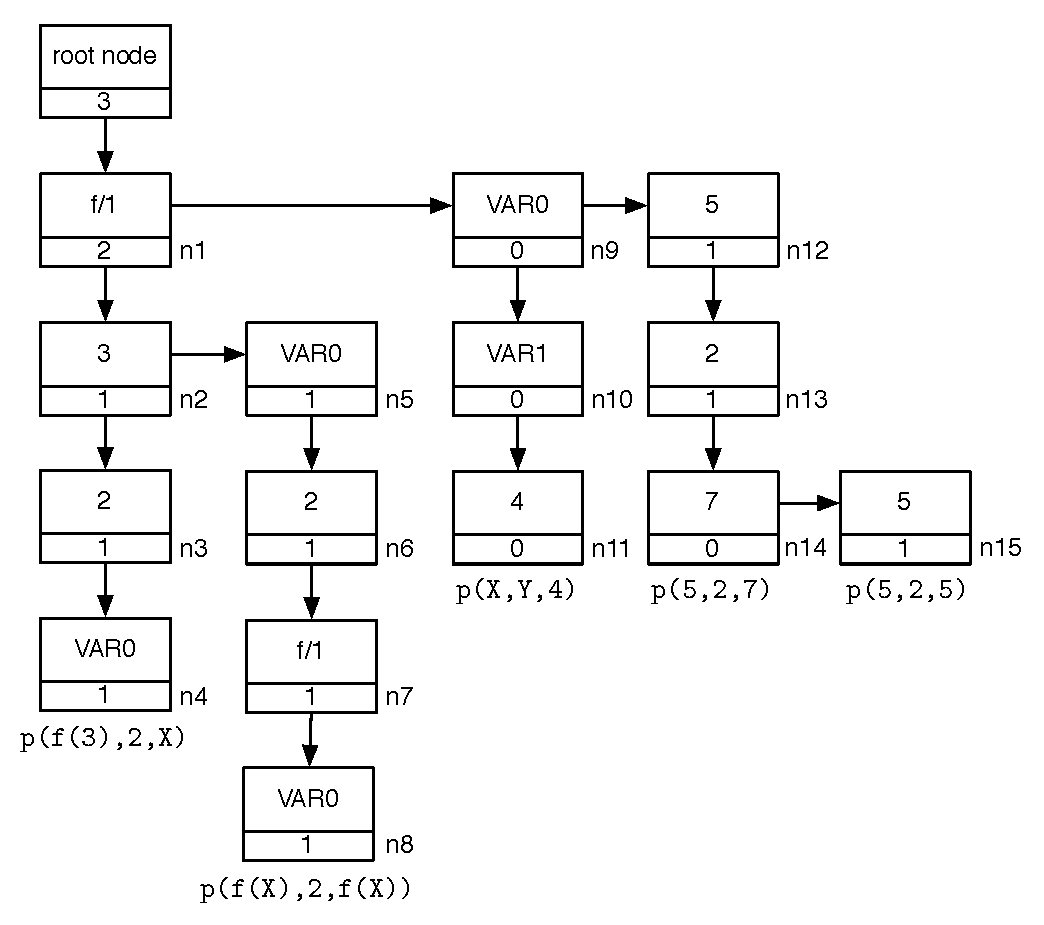
\includegraphics[scale=0.6]{example_trie}
\caption{An example subgoal trie with three evaluating subgoals.}
\label{fig:example_trie}
\end{figure}

Next, we pop the \texttt{X} variable from the term stack and inspect the linked
list of nodes $n1$, $n9$ and $n12$. Because \texttt{X} is a variable term we can potentially
match this term with any node with $\textbf{in\_eval} > 0$. We thus match \texttt{X} against
the symbol \texttt{f/1} from node $n1$ by constructing a new \texttt{f/1} functor
into the heap and pushing a new variable (the functor argument) into the term stack.
Figure~\ref{fig:data_structs1} shows the configuration of the data structures at this point.
Notice that the term log stack now contains the \texttt{X} variable and
the register H now points to the next free heap cell.
Before descending into node $n2$, we need to push the alternative node $n12$ into the choice
point stack. Note that node $n9$ cannot be used as an alternative because no
evaluating subgoals exist in that trie branch.

Next, we pop the unbound functor argument from the term stack and we match it
against the symbol \texttt{3} from node $n2$. Node $n5$ is pushed into the choice
point stack, and we now have the following stack configuration: \texttt{[$n12,n5$]}.
We then descend into node $n3$, where the next term from the term stack, \texttt{2},
matches the trie symbol \texttt{2}. Here, there are no alternative nodes to explore,
and matching proceeds to node $n4$.

In node $n4$ we pop the \texttt{X} variable from the term stack, that when dereferenced,
points to the constructed \texttt{f/1} functor on the heap. As we cannot match ground
terms, such as \texttt{f/1}, with trie variables, the process fails. We then pop the
the top frame of the choice point stack and search is resumed at
node $n5$. The choice point stack now has the following configuration: \texttt{[$n12$]}.
Because we backtracked to try node $n5$, the term stack is restored with the functor
argument, the constant \texttt{2} and the \texttt{X} variable. In node $n5$, the unbound
functor argument is popped from the term stack and is made to point to the index 0 of the
variable enumerator vector, because the trie symbol is the \texttt{VAR0} trie variable.
We then descend into node $n6$, where matching succeeds and then we arrive at node $n7$.
Figure~\ref{fig:data_structs2} presents the configuration of the auxiliary data structures
at this point. Notice that the variable at the $12^{th}$ cell now points to a variable
enumerator position and that the HB register points to the $11^{th}$ cell on the heap, which
corresponds to the value of the H register when we pushed the top choice point frame on the
choice point stack (node $n12$).

\begin{figure}
   \centering
   \subfloat[][Before descending in node $n2$.]{%
      \label{fig:data_structs1}%
      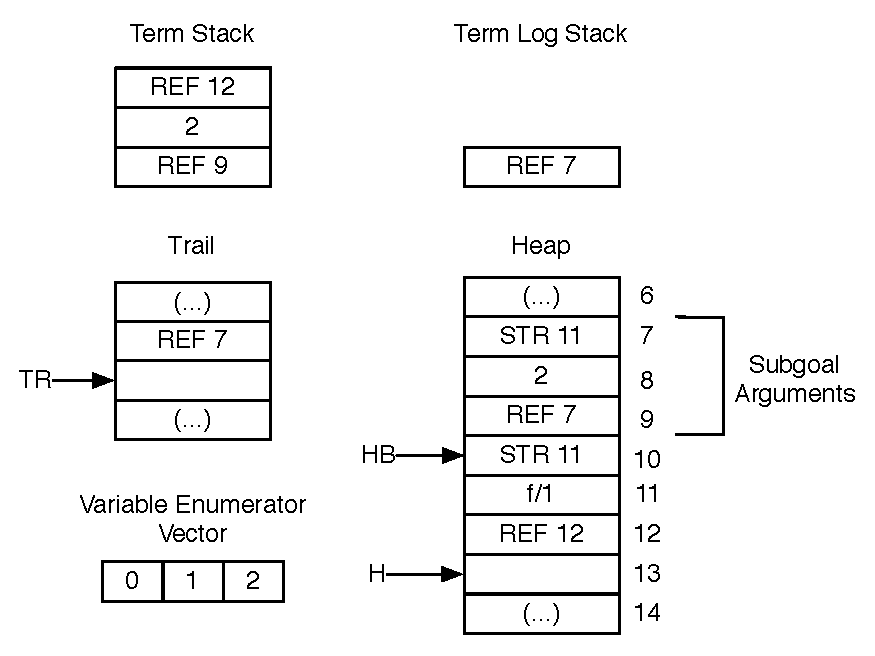
\includegraphics[scale=0.6]{data_structs1.pdf}}%
   \qquad
   \subfloat[][After descending in node $n7$.]{%
      \label{fig:data_structs2}%
      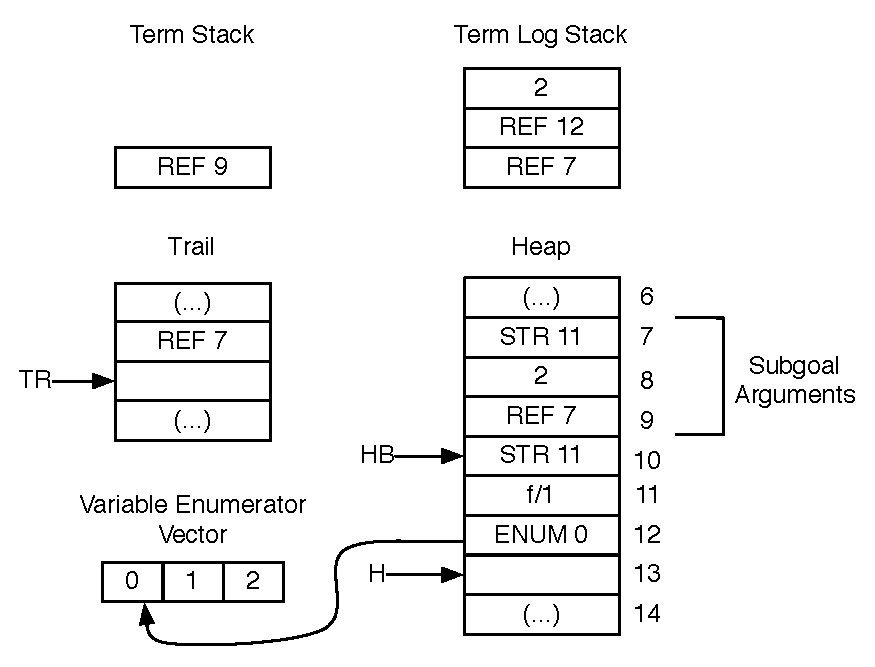
\includegraphics[scale=0.6]{data_structs2.pdf}} \\

   \caption{Auxiliary data structures configuration.}
   \label{fig:data_structs}
\end{figure}

Node $n7$ contains the functor \texttt{f/1} and the next term from the term stack is the
\texttt{X} variable that is bound to the functor \texttt{f/1} created on the heap. Matching
therefore succeeds and we get into node $n8$. In node $n8$ we have the trie variable \texttt{VAR0}
and a variable that is in the variable enumerator vector. Because they both correspond to the index 0,
matching succeeds and a subsumed subgoal is found: \texttt{p(f(X),2,f(X))}.

Next, we pop the top choice point frame from the choice point stack and search is thus resumed
at node $n12$. The term stack is restored to its initial state and the choice point stack is
now empty. Node $n12$ contains the trie symbol \texttt{5} that matches the term variable \texttt{X}
by bounding \texttt{X} to \texttt{5}. Execution proceeds to node $n13$ where the trie symbol
\texttt{2} matches the constant term \texttt{2}. We descend again, now to node $n14$. Here,
only node $n15$ can be used. We then pop the variable \texttt{X} from the term stack that is a
bound to the constant \texttt{5} and matches the trie symbol \texttt{5}. A new
subsumed subgoal is thus found: \texttt{p(5,2,5)}. Finally, as there are no more alternatives,
the algorithm ends and returns the two found subgoals. 

\section{Implementation Details}

In this section we describe some details of the implementation that were not described
in the previous sections, but are still important to understand how RCS was implemented.

\subsection{Subgoal Dependency Tree}

As we have already seen, we build a subgoal dependency tree for generator nodes
in order to construct the call structure of tabled subgoals. We use the \texttt{top\_gen}
field to link internal generator subgoals to the top subgoal.
Hence, we can use the subgoal dependency tree to know if the subgoal $A$ is internal
to the subgoal $B$. To know this, we traverse the \texttt{top\_gen} links until:
(1) subgoal $B$ is reached, thus $A$ is internal to $B$; we reach an older subgoal
than $B$, therefore $A$ is not internal to $B$. We use $B$'s generator choice point
as the threshold for abandoning search and declaring $A$ external of $B$.
Figure~\ref{fig:is_internal_subgoal_frame} presents the pseudo-code for the
\texttt{is\_internal\_subgoal\_frame} function.

\begin{figure}[ht]
\begin{Verbatim}
is_internal_subgoal_frame(target_fr, subgoal_fr, min) {
  if (target_fr == subgoal_fr)
    return TRUE
  
  sg_fr = top_gen(subgoal_fr)
  
  while (sg_fr && younger_or_equal(generator_cp(sg_fr), min))
    if (sg_fr == target_fr)
      return TRUE
    
    sg_fr = top_gen(sg_fr)
  
  return FALSE
}
\end{Verbatim}
\caption{Pseudo-code for function \texttt{is\_internal\_subgoal\_frame}.}
\label{fig:is_internal_subgoal_frame}
\end{figure}

We also extended the dependency frame data structure with a \textbf{top\_gen} field.
Hence, we can compute if a consumer node is internal to another subgoal by calling
the \texttt{is\_internal\_subgoal\_frame} frame above with the dependency frame's top
subgoal frame.

For both cases, the value of the \textbf{top\_gen} field is initialized with the value
of a global variable called \texttt{TOP\_GEN}. This variable is used in various
situations: (1) when a tabled subgoal call creates a generator node we set the
new subgoal frame's \textbf{top\_gen} field to \texttt{TOP\_GEN} and then update
\texttt{TOP\_GEN} to the new subgoal frame; (2) when the new answer tabled operation
is executed we set \texttt{TOP\_GEN} to the value of the subgoal frame's \textbf{top\_gen}
field; (3) when a consumer node is created (and the respective dependency frame) we
use the \texttt{TOP\_GEN} value to set the dependency frame's \textbf{top\_gen} field;
(4) finally, when a consumer node is resumed we set \texttt{TOP\_GEN} to the value
of the dependency frame's \textbf{top\_gen} field.

\subsubsection{Faster External or Internal Test}

While the previous mechanism works pretty well for most cases, it is possible to
implement a faster internal/external test for subgoals that are currently running,
e.g, to test if the more general subgoal is internal or external to a target subsumed
subgoal.

This mechanism extends each subgoal frame with two new fields: \textbf{start\_code}
and \textbf{end\_code}, that initially are standard WAM variables.
The \textbf{start\_code} field is bound to an arbitrary value when the subgoal starts
executing and unbound when the subgoal backtracks, therefore allowing us to detect
if the subgoal is in the current branch. The \textbf{end\_code} field is bound
when a new answer is found, i.e., when the code has reached the end of a program
clause, thus allowing us to easily detect if a pruned subgoal is external or external.

\subsection{Transforming Consumers Into Generators}

In order to be able to transform a consumer node into a retroactive node and then into a generator node,
all consumer choice points are allocated, by default, as generator choice points.

A generator choice points extends a WAM choice point with two fields:
\textbf{sg\_fr}, a pointer to the subgoal frame; \textbf{dep\_fr}, a pointer to a dependency frame,
if evaluating using local scheduling. Allocated along the generator choice point we also have the answer
template and the subgoal arguments. In order for the consumer choice to be the same size as the
generator choice point, we extended the consumer choice point with the \textbf{sg\_fr} field and
the subgoal arguments are also pushed into the local stack.

\subsection{Reference Counting}

We extended the subgoal frame data structure with a field called \textbf{num\_deps}. This field
counts the number of dependency frames dependent on this subgoal. Therefore, while updating
external consumers to transform them into retroactive nodes we count the number of external consumers
already processed, and thus we can exit early when the count reaches the target number. This speedups
the pruning process because we known when all external consumers were already processed.

For subsumptive generator subgoal frames, we extended them with an extra field called \textbf{num\_sub\_deps}, that
counts the number of subsumed consumers. By knowing how many variant consumers and subsumed consumers we
have for a generator we can decide more efficiently when to transform external consumers and if we
need to transform subsumed consumer nodes to use a generator subgoal frame, if no variant external consumers
exist anymore.

\subsection{Computing Stack Limits}

One important input parameter of pruning are the choice points relevant to the
computation of target subgoal. We estimate this parameter by first storing the
address of the generator choice point as the upper limit, and the lower limit is
updated to the lowest value of \textbf{B\_FZ} or \textbf{B} when: (1) a new answer is
generated, (2) a new clause is executed, or (3) completion is attempted. While this
is a simple approach, some parts of the local stack can belong to an
\textit{external generator}. This can happen when an external consumer
suspends. Updating the bottom limit to \textbf{B\_FZ} allow us to cover areas of
the stack that were frozen during evaluation of the subgoal.

\subsection{Data Structure Modifications}

To be able to set a predicate to use retroactive call subsumption, we added another flag to the
\textbf{mode\_flag} bit field of the table entry. In addition to the flags \textbf{variant} and 
\textbf{subsumptive}, \textbf{retroactive} is also available.

For the dependency frame, we extended it with the bit field \textbf{flags}. Among other things,
one bit marks if the corresponding consumer is a potential lost consumer, therefore if the completion
operation will attempt to resume the consumer, it will check first for that bit flag to execute
retroactive resolution in order to transform the node into a generator.

The retroactive subgoal frame was extended with a \textbf{try\_answer} field. This field is used
to consume the available answers from the answer trie that are relevant to the subgoal
before attempting to execute the predicate clauses.

We extended both the subgoal and the dependency frame with two new fields, \textbf{prev} and
\textbf{next}, that are used to double link the frames on the respective stacks. These pointers
make the operation of removing a frame from the respective stack more efficient.

\subsection{Tabling Operations}

The most important modifications to tabling operations were done in the tabled subgoal call and
completion operations. For the tabled subgoal call operation (Figure~\ref{fig:tabled_subgoal_call_retro})
we distinguish the new retroactive evaluation method by calling the procedure \texttt{retroactive\_subgoal\_search}.
When we have a new generator call, after storing the
generator node, we collect the running subsumed subgoals, we mark ourselves as a running subgoal, and
then we prune the found subgoals by calling \texttt{prune\_subgoal\_list}.
Next, we attempt to collect new relevant answers from the STST with
\texttt{collect\_available\_retroactive\_answers} and if the subgoal frame contains any answer
we load them by using the \texttt{table\_try\_answer} instruction.

The tabled subgoal call operation must also check if the subgoal frame is in the pruned state. Here,
we simply load all the available answers and then call the \texttt{table\_try\_answer} instruction,
which will load all the available answers and then execute the program clauses.

\begin{figure}[ht]
\begin{Verbatim}
tabled_subgoal_call(table_entry, arguments) {
  call_trie = call_trie(table_entry)
  
  if(method(table_entry) == VARIANT)
    subgoal_frame = variant_subgoal_search(call_trie, arguments)
  else if (method(table_entry) == SUBSUMPTIVE)
    subgoal_frame = subsumptive_subgoal_search(call_trie, arguments)
  else if (method(table_entry) == RETROACTIVE) // NEW
    subgoal_frame = retroactive_subgoal_search(call_trie, arguments)
  
  if (is_new_generator_call(subgoal_frame))
    store_generator_node(table_entry, arguments, subgoal_frame)
    if (type(subgoal_frame) == RETROACTIVE_GENERATOR)
      subgoals = collect_subsumed_subgoals(arguments, call_trie)
      increment_in_eval(subgoal_frame)
      prune_subgoal_list(subgoal_frame, subgoals)
      collect_available_retroactive_answers(subgoal_frame)
      if (get_first_answer(subgoal_frame))
        // consume pre stored answers
        first = get_first_answer(subgoal_frame)
        load_answer_from_trie(first)
        try_answer(subgoal_frame) = first
        CP_AP(B) = table_try_answer
        goto continuation_instruction()
  else if (state(subgoal_frame) == pruned) // NEW
    // consume pre stored answers
    state(subgoal_frame) = evaluating
    first = get_first_answer(subgoal_frame)
    load_answer_from_trie(first)
    try_answer(subgoal_frame) = first
    CP_AP(B) = table_try_answer
    goto continuation_instruction()
  else if (is_new_consumer_call(subgoal_frame))
    // (...)
  else
    // (...)
}
\end{Verbatim}
\caption{Pseudo-code for the new tabled subgoal call operation.}
\label{fig:tabled_subgoal_call_retro}
\end{figure}

When trying to complete by traversing the dependency space for unconsumed answers, we must
also check for lost consumers. These consumers must be restarted as generators in order for
computation be completed. Figure~\ref{fig:completion_operation_retro} presents the new completion
operation. Note that we detect a lost consumer we call the \texttt{retroactive\_resolution}
instruction in order to restart the consumer.

\begin{figure}[ht]
\begin{Verbatim}
completion(generator) {
  if (is_leader_node(generator))
    df = TOP_DEP_FR
    while (younger_than(cons_cp(df), generator))
      // NEW
      if (is_lost_consumer(df))
        consumer = cons_cp(df)
        CP_B(consumer) = generator
        restore_bindings(CP_TR(generator), CP_TR(consumer))
        goto retroactive_resolution(consumer)
      cont = get_next_answer_continuation(dep_fr)
      if (cont)
        // unconsumed answers
        back_cp(df) = generator
        consumer = cons_cp(df)
        restore_bindings(CP_TR(generator), CP_TR(consumer))
        goto answer_resolution(consumer)
      df = next(df)
    perform_completion()
    adjust_freeze_registers()
  backtrack_to(CP_B(generator))
}
\end{Verbatim}
\caption{Pseudo-code for the new completion operation.}
\label{fig:completion_operation_retro}
\end{figure}
